\documentclass[12pt,a4paper]{ctexart}

% ========== 页面与字体 ==========
\usepackage{geometry}
\geometry{left=2.6cm,right=2.6cm,top=2.5cm,bottom=2.5cm}

\usepackage{fontspec}
\IfFontExistsTF{Times New Roman}{\setmainfont{Times New Roman}}{\setmainfont{TeX Gyre Termes}}
\IfFontExistsTF{Consolas}{\setmonofont{Consolas}}{\setmonofont{Courier New}}

\usepackage{setspace}
\onehalfspacing
\setlength{\parindent}{2em}
\setlength{\parskip}{0.25em}
\sloppy
\emergencystretch=2em

% ========== 数学与图表 ==========
\usepackage{amsmath,amsthm}
\usepackage{unicode-math}
\IfFontExistsTF{Cambria Math}{\setmathfont{Cambria Math}}{}
\usepackage{graphicx}
\usepackage{booktabs}
\usepackage{array}
\usepackage{tabularx}
\usepackage{caption}
\usepackage{subcaption}
\usepackage{float}
\newcolumntype{Y}{>{\raggedright\arraybackslash}X}
\setlength{\tabcolsep}{4pt}
\graphicspath{{figures/}}

% ========== 列表 ==========
\usepackage{enumitem}
\setlist{itemsep=0.2em,topsep=0.4em}

% ========== 颜色与链接 ==========
\usepackage{xcolor}
\definecolor{mainblue}{HTML}{2F5597}
\definecolor{lightblue}{HTML}{EAF2FF}
\definecolor{darkgray}{HTML}{333333}

\usepackage[
    colorlinks=true,
    linkcolor=mainblue,
    citecolor=mainblue,
    urlcolor=mainblue
]{hyperref}

% ========== 标题样式 ==========
\usepackage{titlesec}
\titleformat{\section}{\Large\bfseries\color{mainblue}}{\thesection}{0.8em}{}
\titleformat{\subsection}{\large\bfseries\color{darkgray}}{\thesubsection}{0.8em}{}
\titleformat{\subsubsection}{\normalsize\bfseries}{\thesubsubsection}{0.8em}{}

% ========== 页眉页脚 ==========
\usepackage{fancyhdr}
\pagestyle{fancy}
\setlength{\headheight}{14.5pt}
\fancyhf{}
\fancyhead[L]{\color{mainblue}实物控制实验报告}
\fancyhead[R]{\color{mainblue}\leftmark}
\fancyfoot[C]{\thepage}
\renewcommand{\headrulewidth}{0.4pt}
\renewcommand{\footrulewidth}{0pt}

% ========== 代码样式 ==========
\usepackage{listings}
\lstset{
    basicstyle=\ttfamily\small,
    keywordstyle=\color{mainblue}\bfseries,
    commentstyle=\color{gray},
    stringstyle=\color{teal},
    numbers=left,
    numberstyle=\tiny\color{gray},
    frame=single,
    breaklines=true,
    backgroundcolor=\color{lightblue},
    rulecolor=\color{mainblue},
    tabsize=4
}

% ========== 提示框与定理环境 ==========
\usepackage[most]{tcolorbox}
\newtcolorbox{notebox}{
    colback=lightblue,
    colframe=mainblue,
    arc=2mm,
    boxrule=0.8pt,
    left=8pt,
    right=8pt,
    top=6pt,
    bottom=6pt,
    title=\textbf{提示}
}
\newtheorem{theorem}{定理}
\newtheorem{definition}{定义}
\newtheorem{example}{例}

% ========== 文档信息 ==========
\title{
    \vspace{1.2cm}
    \Huge \textbf{\color{mainblue} H1 右髋-右膝输入域 EID 与 Preview-MPC 实物实验报告 }\\[0.5em]
    \Large Unitree H1 右髋-右膝实物控制实验
}
\author{实验日期：2026-06-23\\[0.25em]
实验对象：Unitree H1 右髋俯仰关节与右膝关节\\[0.25em]
}
\date{\today}

\begin{document}

\maketitle
\thispagestyle{empty}

\begin{abstract}
本文报告 Unitree H1 右髋俯仰与右膝关节在悬挂或机械保护条件下的第一轮实物实验结果。实验对象为\textbf{包含解析逆模型的输入域 EID 整体结构}，并与电机位置模式 PD 基线以及 Preview-MPC 参考生成方法进行对比。本文重点回答四个工程问题：EID 整体结构在无扰动低幅双关节运动中是否安全有效；在明确扰动条件下是否改善跟踪与协调误差；Preview-MPC 是否降低参考激励和力矩变化量；以及 $K_o$、$K_u$ 参数对稳定性、误差和力矩代价的影响。

结果显示，EID 整体结构在 P1 无扰动实验中降低髋、膝和协调 RMSE，且未观察到批量运行失败；在 P2-H 髋人工扰动实验中，EID 整体结构的全稳态误差低于 PD，但由于人工扰动未记录开始和结束时间，P2-H 不能作为严格扰动窗口结论。P2D 双关节软件力矩扰动给出了可复现扰动窗口：在 $[+6,-4]\ \mathrm{N\cdot m}$ 平滑力矩脉冲下，EID 整体结构将髋窗口 RMSE 降低 18.2\%、协调窗口 RMSE 降低 6.1\%，但膝窗口 RMSE 上升 10.0\%，且力矩 RMS 与力矩变化量均增加。

Preview-MPC 2 点参考在 P3 中显著降低参考加速度、参考 jerk 和力矩变化量，代价是髋/膝跟踪 RMSE 小幅上升。P4D 参数扫描显示，O0 在软件扰动下无法覆盖完整扰动窗口，O4/O5 均能稳定完成；增大 $K_o$ 可降低扰动窗口误差，而增大 $K_u$ 几乎不改善窗口 RMSE，只放大 $\eta_u$ 活动量。

本轮结论的边界是：P2D/P4D 支持\textbf{输入端等效扰动}下的实物结论，但不能替代真实外部物理接触力实验。短期后续工作应先基于现有 P2D/P4D 日志完成频谱分析与恢复段统计，并并行推进控制器机理仿真，以明确力矩变化量增加的频段来源、扰动撤除后的回稳行为以及 EID 整体结构的主要收益通道。
\end{abstract}

\newpage
\tableofcontents
\newpage

\section{实验目的}


第一轮实物实验只回答以下四个工程问题。

\begin{table}[htbp]
\centering
\footnotesize
\caption{第一轮工程问题与回答状态}
\begin{tabularx}{\textwidth}{YYYY}
\toprule
编号 & 问题 & 对应实验 & 本轮回答状态 \\
\midrule
Q1 & EID 整体结构在无扰动低幅髋膝运动中是否安全有效 & P1 & 已回答 \\
Q2 & EID 整体结构在扰动下是否降低误差，且不增加协调误差 & P2-H、P2D & \textbf{部分回答：软件输入端等效扰动已回答；真实物理外扰未回答} \\
Q3 & Preview-MPC 是否降低参考加速度、参考 jerk 和力矩变化量，同时不明显破坏跟踪 & P3 & 已回答 \\
Q4 & $K_o$ 与 $K_u$ 如何影响 EID 整体结构的稳定性、误差和力矩代价 & P4、P4D & 已回答本轮无扰动和软件扰动条件；尚不是跨工况最优参数 \\
\bottomrule
\end{tabularx}
\end{table}


\section{控制算法概述}


本节给出当前实验所使用控制器的核心结构，便于读者理解后续参数和指标。完整递推关系见控制算法说明，本文只保留与实验结论直接相关的部分。本文中的 EID 均指\textbf{包含解析逆模型的输入域 EID 整体结构}，而不是单独的估计模块。

\begin{figure}[htbp]
\centering
\includegraphics[width=0.92\textwidth]{figures/control_algorithm_block_diagram.png}
\caption{输入域 EID 整体结构框图。参考生成器提供当前控制周期和下一控制周期的参考位置、参考速度；解析逆模型给出标称前馈力矩 $u_k^*$；EID 估计量经 $K_u$ 映射为输入端补偿 $\eta_{u,k}$；最终控制律围绕中心反馈状态 $\bar{x}_k=\hat{x}_k+\eta_k$ 构造。当前实现中，EID 更新使用实测状态与中心反馈状态之间的残差 $x_k-\bar{x}_k$，而不是实测状态与标称预测状态之间的残差 $x_k-\hat{x}_k$。}
\end{figure}


\subsection{参考生成与最终参考}


实验中的轨迹首先由正弦策略参考产生。该原始策略参考只描述理想运动目标，不一定直接作为电机每个控制周期的最终参考。控制器还会经过插值、Preview-MPC 或启动混入处理，得到最终参考。

时序图中三条曲线的含义如下。

\begin{table}[htbp]
\centering
\footnotesize
\caption{时序图曲线说明}
\begin{tabularx}{\textwidth}{YYY}
\toprule
曲线 & 含义 & 在图中的样式 \\
\midrule
原始策略参考 & 由正弦策略直接生成的理想位置和速度 & 黑色点线 \\
最终参考 & 控制器实际使用的参考，包含插值、Preview-MPC 和启动混入 & 蓝色虚线 \\
实测状态 & 机器人关节反馈的位置和速度 & 橙色实线 \\
\bottomrule
\end{tabularx}
\end{table}


启动混入用于避免控制开始瞬间从当前关节角直接跳到正弦轨迹位置。本轮实验的启动混入时间为 3.0 s，因此时序图前 3 s 中，最终参考会从实测初始状态平滑接入原始策略参考。

Preview-MPC 是参考生成层，不是力矩控制器。其作用是在策略层低频给出离散位置点时，为每个 $T_s=0.002\ \mathrm{s}$ 控制周期生成平滑的 $q^*$、$\dot{q}^*$ 和 $\ddot{q}^*$。策略参考采样周期为

\[
T_p=0.05\ \mathrm{s}
\]

单个策略周期内的控制步数为

\[
N_p=\mathrm{round}\left(\frac{T_p}{T_s}\right)
\]

若使用 $n$ 个预览点，则优化窗口长度为

\[
N_h=nN_p
\]

P3 中的 \texttt{preview2} 对应 $n=2$，即第一个策略点作为硬目标，第二个策略点作为软预览目标。Preview-MPC 对每个关节独立求解，状态为

\[
z_i=
\begin{bmatrix}
q_i\\
\dot q_i\\
\ddot q_i
\end{bmatrix}
\]

优化变量为窗口内 jerk 序列

\[
J=
\begin{bmatrix}
j_0 & j_1 & \cdots & j_{N_h-1}
\end{bmatrix}^{T},
\qquad
j_i=\dddot q_i
\]

在每个控制步内假设 jerk 为常值，离散运动学递推为

\[
\ddot q_{i+1}=\ddot q_i+T_s j_i
\]

\[
\dot q_{i+1}
=
\dot q_i+T_s\ddot q_i+\frac{1}{2}T_s^2j_i
\]

\[
q_{i+1}
=
q_i+T_s\dot q_i+\frac{1}{2}T_s^2\ddot q_i+\frac{1}{6}T_s^3j_i
\]

设预览到的策略位置点为 $q_1^p,\ldots,q_n^p$，优化问题可概括为

\[
\min_J L_\mathrm{mpc}
\]

其中

\[
\begin{aligned}
L_\mathrm{mpc}
=&
\sum_{i=0}^{N_h-1}
\left(
w_j j_i^2
+w_v\dot q_i^2
+w_a\ddot q_i^2
\right)\\
&+
\sum_{\ell=2}^{n}
w_p
\left(q_{\ell N_p}-q_\ell^p\right)^2
+w_{Tv}\dot q_{N_h}^2
+w_{Ta}\ddot q_{N_h}^2
\end{aligned}
\]

并满足硬约束

\[
q_{N_p}=q_1^p
\]

求解后只执行第一个策略周期内的参考，下一策略周期重新读取预览点并再次规划。与零速五次样条相比，Preview-MPC 的工程目的不是提高反馈增益，而是提前分配速度、加速度和 jerk，从而降低参考高阶激励和力矩变化量。

\subsection{输入域 EID 控制律核心}


对每个关节，控制器维护一个标称预测状态和一个 EID 估计量。标称预测状态来自单关节动力学模型。EID 估计量用于修正标称预测状态，并通过 $K_u$ 映射为输入端补偿。本文不把 $\eta_k$ 或 $\eta_u$ 直接解释为真实外力或真实外部扰动力矩，而是将其作为 EID 整体结构内部的状态修正量和输入补偿量。标称预测状态与 EID 估计量相加后得到中心反馈状态。

核心关系可写为：

\[
\bar{x}_k=\hat{x}_k+\eta_k
\]

其中，$\hat{x}_k$ 为标称预测状态，$\eta_k$ 为 EID 估计量，$\bar{x}_k$ 为中心反馈状态。

EID 估计量通过 $K_u$ 映射成输入端力矩补偿：

\[
\eta_{u,k}=k_{u,q}\eta_{q,k}+k_{u,\dot q}\eta_{\dot q,k}
\]

解析逆模型先根据当前参考和下一步参考计算标称前馈力矩 $u_k^*$。EID 整体结构再从前馈力矩中扣除输入补偿项：

\[
u_{k,\mathrm{ff}}=u_k^*-\eta_{u,k}
\]

当前实现的核心控制律可写为

\[
u_k
=
u_k^*
-\eta_{u,k}
+K(r_k-\bar{x}_k)
\]

其中 $K=[k_p\ k_d]$。该式表明，最终力矩由解析逆模型前馈、输入端补偿以及围绕中心反馈状态的 PD 修正共同构成。$K_o$ 决定 EID 估计量对状态残差的响应强度；$K_u$ 决定估计量映射到输入补偿力矩的强度。

因此，$K_o$ 更接近“估计器增益”，$K_u$ 更接近“补偿强度”。$K_o$ 过小会导致估计通道不足，$K_o$ 或 $K_u$ 过大则可能增加力矩活动、噪声敏感性或高频成分。

\section{实验设置与参数}


\subsection{关节与执行条件}


本轮只启用两个下肢关节。所有实验均应理解为悬挂或机械保护条件下的台架实验，而不是自由站立实验。

\begin{table}[htbp]
\centering
\footnotesize
\caption{关节与观察量}
\begin{tabularx}{\textwidth}{YYYY}
\toprule
关节 & joint id & 角色 & 主要观察量 \\
\midrule
RightHipPitch & 1 & 髋俯仰跟踪；P2-H 扰动对象 & 髋误差、髋力矩、协调误差 \\
RightKnee & 2 & 膝关节跟踪；非受扰通道观察 & 膝误差、膝力矩、协调误差 \\
\bottomrule
\end{tabularx}
\end{table}


\subsection{通用控制与安全参数}


\begin{table}[htbp]
\centering
\footnotesize
\caption{通用控制与安全参数}
\begin{tabularx}{\textwidth}{@{}p{0.16\textwidth}p{0.25\textwidth}p{0.31\textwidth}p{0.13\textwidth}@{}}
\toprule
符号 & 含义 & 代码符号 & 本轮取值 \\
\midrule
$T_s$ & 控制周期 & \texttt{control\_dt} & 0.002 s \\
$T_p$ & 策略参考采样周期 & \texttt{policy\_dt} & 0.05 s \\
$t_\mathrm{blend}$ & 启动参考混入时间 & \texttt{startup\_blend\_duration\_s} & 3.0 s \\
$\tau_{\max}$ & 命令力矩限幅 & \texttt{tau\_limit} & 100 N·m \\
$\dot{\tau}_{\max}$ & EID 力矩变化率限制 & \texttt{tau\_slew\_rate} & 100 N·m/s \\
$\dot q_\mathrm{trip}$ & 实测速度硬停阈值 & \texttt{measured\_speed\_trip} & 6.0 rad/s \\
$k_{p,\mathrm{hold}}$ & safe-hold 位置增益 & \texttt{safe\_hold.kp} & 6.0 \\
$k_{d,\mathrm{hold}}$ & safe-hold 速度增益 & \texttt{safe\_hold.kd} & 1.0 \\
\bottomrule
\end{tabularx}
\end{table}


\subsection{关节模型与限幅参数}


\begin{table}[htbp]
\centering
\footnotesize
\caption{关节模型与限幅参数}
\begin{tabularx}{\textwidth}{@{}p{0.16\textwidth}p{0.18\textwidth}p{0.23\textwidth}p{0.13\textwidth}p{0.13\textwidth}@{}}
\toprule
符号 & 含义 & 代码符号 & RightHipPitch，ID 1 & RightKnee，ID 2 \\
\midrule
$J_\mathrm{eff}$ & 等效惯量 & \texttt{plant.Jeff} & 1.00508532 & 0.2501484 \\
$b$ & 阻尼系数 & \texttt{plant.b} & 1.0 & 1.0 \\
$A$ & 重力项 $\sin q$ 系数 & \texttt{plant.gravityA} & 15.7100627 & 4.14117407 \\
$B$ & 重力项 $\cos q$ 系数 & \texttt{plant.gravityB} & 2.79723089 & -2.09365203 \\
$\tau_0$ & 常值力矩偏置 & \texttt{plant.tau0} & 0.0 & 0.0 \\
$q_{\min}$ & 位置下界 & \texttt{joint\_limits.q\_min} & -3.14 rad & -0.26 rad \\
$q_{\max}$ & 位置上界 & \texttt{joint\_limits.q\_max} & 2.53 rad & 2.05 rad \\
$\dot q_{\max}$ & 速度上界 & \texttt{joint\_limits.dq\_max} & 23 rad/s & 14 rad/s \\
$\tau_{\max}$ & 实际命令力矩限幅 & \texttt{joint\_limits.tau\_max} & 100 N·m & 100 N·m \\
$\tau_{\max,\mathrm{plant}}$ & 模型力矩上界 & \texttt{plant.tau\_max} & 200 N·m & 300 N·m \\
\bottomrule
\end{tabularx}
\end{table}


\subsection{控制器参数}


PD 与 EID 整体结构的反馈增益均使用 $k_p=120.0$、$k_d=5.0$。PD 通过电机位置模式下发参考位置、参考速度和电机侧 $k_p/k_d$；EID 整体结构通过输入域补偿计算命令力矩。因此，力矩代价比较优先使用执行器反馈或估计力矩 $\tau_\mathrm{est}$，而不是 \texttt{tau\_cmd}。

\begin{table}[htbp]
\centering
\footnotesize
\caption{控制器基准参数}
\begin{tabularx}{\textwidth}{YYYY}
\toprule
符号 & 含义 & 代码符号 & 基准值 \\
\midrule
$k_p$ & 位置反馈增益 & \texttt{kp} & 120.0 \\
$k_d$ & 速度反馈增益 & \texttt{kd} & 5.0 \\
$k_{o,q}$ & EID 位置观测器增益 & \texttt{observer\_gain\_q} & 0.8 \\
$k_{o,\dot q}$ & EID 速度观测器增益 & \texttt{observer\_gain\_dq} & 0.2 \\
$k_{u,q}$ & EID 位置输入补偿增益 & \texttt{ku\_q} & 12.0 \\
$k_{u,\dot q}$ & EID 速度输入补偿增益 & \texttt{ku\_dq} & 1.0 \\
$\alpha$ & EID 估计低通滤波系数 & \texttt{filter\_alpha} & 0.85 \\
\bottomrule
\end{tabularx}
\end{table}


P4 使用相对缩放扫描 $K_o$ 与 $K_u$。

\begin{table}[htbp]
\centering
\footnotesize
\caption{EID 增益扫描参数}
\begin{tabularx}{\textwidth}{YYYYYYYY}
\toprule
扫描 & 组别 & $K_o$ 缩放 & $K_u$ 缩放 & $k_{o,q}$ & $k_{o,\dot q}$ & $k_{u,q}$ & $k_{u,\dot q}$ \\
\midrule
$K_o$ & O0 & 0.00 & 1.00 & 0.0 & 0.00 & 12.0 & 1.00 \\
$K_o$ & O1 & 0.25 & 1.00 & 0.2 & 0.05 & 12.0 & 1.00 \\
$K_o$ & O2 & 0.50 & 1.00 & 0.4 & 0.10 & 12.0 & 1.00 \\
$K_o$ & O3 & 0.75 & 1.00 & 0.6 & 0.15 & 12.0 & 1.00 \\
$K_o$ & O4 & 1.00 & 1.00 & 0.8 & 0.20 & 12.0 & 1.00 \\
$K_o$ & O5 & 1.25 & 1.00 & 1.0 & 0.25 & 12.0 & 1.00 \\
$K_u$ & U1 & 1.00 & 0.50 & 0.8 & 0.20 & 6.0 & 0.50 \\
$K_u$ & U2 & 1.00 & 0.75 & 0.8 & 0.20 & 9.0 & 0.75 \\
$K_u$ & U3 & 1.00 & 1.00 & 0.8 & 0.20 & 12.0 & 1.00 \\
$K_u$ & U4 & 1.00 & 1.25 & 0.8 & 0.20 & 15.0 & 1.25 \\
\bottomrule
\end{tabularx}
\end{table}


\subsection{参考轨迹与实验矩阵}


\begin{table}[htbp]
\centering
\footnotesize
\caption{参考轨迹与实验矩阵}
\begin{tabularx}{\textwidth}{YYYYYYYY}
\toprule
实验 & 控制方案 & 相位关系 & 频率 Hz & 髋中心/幅值 rad & 膝中心/幅值 rad & 扰动 & 重复次数 \\
\midrule
P1 & PD vs EID & 同相 & 0.86112 & -0.300 / 0.1859 & 0.500 / 0.232375 & 无 & 每组 5 \\
P2-H & PD vs EID & 反相 & 0.80000 & -0.300 / 0.22308 & 0.500 / 0.278850 & 髋人工扰动 & 每组 5 \\
P2D & PD vs EID & 反相 & 0.80000 & -0.300 / 0.22308 & 0.500 / 0.278850 & 双关节软件力矩扰动 & 每组 5 \\
P3 & quintic vs preview2，PD & 同相 & 0.80000 & -0.300 / 0.1859 & 0.500 / 0.232375 & 无 & 每组 2 \\
P4 $K_o$ & EID & 反相 & 0.80000 & -0.300 / 0.22308 & 0.500 / 0.278850 & 无 & 每组 3 \\
P4 $K_u$ & EID & 反相 & 0.80000 & -0.300 / 0.22308 & 0.500 / 0.278850 & 无 & 每组 3 \\
P4D $K_o$ & EID & 反相 & 0.80000 & -0.300 / 0.22308 & 0.500 / 0.278850 & 双关节软件力矩扰动 & 每组 3 \\
P4D $K_u$ & EID & 反相 & 0.80000 & -0.300 / 0.22308 & 0.500 / 0.278850 & 双关节软件力矩扰动 & 每组 3 \\
\bottomrule
\end{tabularx}
\end{table}


P3 中 quintic 指零速五次样条参考，preview2 指 2 点 Preview-MPC 参考生成。P2-H 中人工扰动只记录了扰动对象和方式，未记录扰动开始/结束时间。

P2D 和 P4D 使用同一个可复现软件力矩扰动。扰动在控制器输出后、最终安全限幅前叠加到命令力矩中：

\[
\tau_d(t)=s(t)
\begin{bmatrix}
+6\\
-4
\end{bmatrix}
\ \mathrm{N\cdot m}
\]

其中第一项对应 RightHipPitch，第二项对应 RightKnee。$s(t)$ 为 half-cosine 平滑矩形窗，$4.0$--$4.2\ \mathrm{s}$ 平滑上升，$4.2$--$5.2\ \mathrm{s}$ 保持，$5.2$--$5.4\ \mathrm{s}$ 平滑下降。该扰动用于验证输入端等效扰动抑制，不等同于外部物理接触力。

\section{概念与指标定义}


为使结果表和图可以独立阅读，本节先定义报告中反复出现的概念。

\begin{table}[htbp]
\centering
\footnotesize
\caption{报告概念定义}
\begin{tabularx}{\textwidth}{YY}
\toprule
概念 & 定义 \\
\midrule
$q$ & 关节位置，单位为 rad \\
$\dot q$ & 关节速度，单位为 rad/s \\
参考 & 控制器希望关节达到的位置和速度 \\
原始策略参考 & 由正弦策略直接计算得到的理想参考 \\
最终参考 & 经过插值、Preview-MPC 和启动混入后，控制器实际使用的参考 \\
实测状态 & 机器人反馈的真实关节位置和速度 \\
PD & 位置-速度反馈控制，使用电机位置模式下发参考位置、参考速度和反馈增益 \\
输入域 EID 整体结构 & 包含解析逆模型前馈、输入端补偿和中心反馈状态 PD 修正的整体控制结构 \\
Preview-MPC & 利用未来参考点生成更平滑参考的预览式参考生成方法 \\
$K_o$ & EID 观测器增益，决定估计量对状态偏差的响应强度 \\
$K_u$ & EID 输入补偿强度，决定估计量转换为补偿力矩的强度 \\
P2-H & P2 中髋关节受到人工轻扰动的子工况 \\
P2D & P2 的软件扰动补充实验，髋膝同时叠加平滑力矩脉冲 \\
P4D & P4 的软件扰动补充扫描，使用与 P2D 相同的力矩脉冲 \\
无扰动扫描 & 不施加外部扰动，只观察参数变化对跟踪、力矩和稳定性的影响 \\
软件力矩扰动 & 在命令侧叠加的等效输入扰动，用于提高扰动时间窗和幅值的可复现性 \\
\bottomrule
\end{tabularx}
\end{table}


RMSE 是均方根误差，用于描述一段时间内误差的平均大小。RMSE 越小，表示该指标越接近参考目标。其计算方式为：

\[
\mathrm{RMSE}=\sqrt{\frac{1}{N}\sum_{i=1}^{N}e(t_i)^2}
\]

单关节跟踪误差表示某个关节的最终参考与实测状态之间的差：

\[
e_j(t)=q_{\mathrm{ref},j}(t)-q_j(t)
\]

协调误差用于描述髋膝相对运动是否保持正确。它不只看单个关节是否跟准，而是看“膝相对髋”的实际角度是否等于“膝相对髋”的参考角度：

\[
e_{\mathrm{coord}}(t)=
\left[q_{\mathrm{knee}}(t)-q_{\mathrm{hip}}(t)\right]
-
\left[q_{\mathrm{ref},\mathrm{knee}}(t)-q_{\mathrm{ref},\mathrm{hip}}(t)\right]
\]

协调 RMSE 就是对 $e_{\mathrm{coord}}(t)$ 计算 RMSE。它用于判断两个关节之间的相对节奏、相位和姿态关系是否被控制器破坏。

力矩相关指标包括 $\tau_\mathrm{est}$ RMS 和 $\Delta \tau_\mathrm{est}$ RMS。$\tau_\mathrm{est}$ 是执行器反馈或估计到的关节力矩，$\tau_\mathrm{est}$ RMS 表示平均力矩负担；$\Delta \tau_\mathrm{est}$ RMS 表示相邻采样点之间力矩变化量的均方根，反映力矩输入是否更粗糙、更活跃。

参考加速度 RMS 和参考 jerk RMS 用于评价参考轨迹平滑性。加速度是速度变化率，jerk 是加速度变化率。二者越小，通常表示参考轨迹越平滑，对执行器的高频激励越少。

\section{数据处理方法}


所有定量结果均使用实验开始后 $t_\mathrm{rel}\ge 3.0\ \mathrm{s}$ 的稳态段，避开启动混入阶段。每个表格中的数值为重复实验的均值；图中的误差线表示重复实验标准差。

P2D 和 P4D 另计算扰动窗口指标。完整扰动窗口定义为 $4.0\le t_\mathrm{rel}<5.4\ \mathrm{s}$，其中 $4.2$--$5.2\ \mathrm{s}$ 为恒定扰动平台段，$5.4$--$7.4\ \mathrm{s}$ 作为恢复观察段。若某次日志没有覆盖完整扰动窗口，该次不用于完整窗口均值，并在结果表中单独标注完整次数。

代表性时序图均从实验开始时刻绘制，即横轴使用 $t_\mathrm{rel}=t-t_0$。时序图中，黑色点线表示原始策略参考，蓝色虚线表示最终参考，橙色实线表示实测状态。

主要指标如下。

\begin{table}[htbp]
\centering
\footnotesize
\caption{主要评价指标}
\begin{tabularx}{\textwidth}{YYY}
\toprule
指标 & 单位 & 用途 \\
\midrule
髋/膝 RMSE & rad & 单关节跟踪精度 \\
协调误差 RMSE & rad & 髋膝相对运动是否被破坏 \\
$\tau_\mathrm{est}$ RMS & N·m & 执行器负担 \\
$\Delta \tau_\mathrm{est}$ RMS & N·m/sample & 力矩粗糙度或输入变化强度 \\
参考加速度 RMS & rad/s² & P3 参考平滑性 \\
参考 jerk RMS & rad/s³ & P3 高阶参考激励 \\
\bottomrule
\end{tabularx}
\end{table}


\section{结果}


\subsection{P1/P2-H：EID 整体结构的稳态跟踪结果}


\begin{figure}[htbp]
\centering
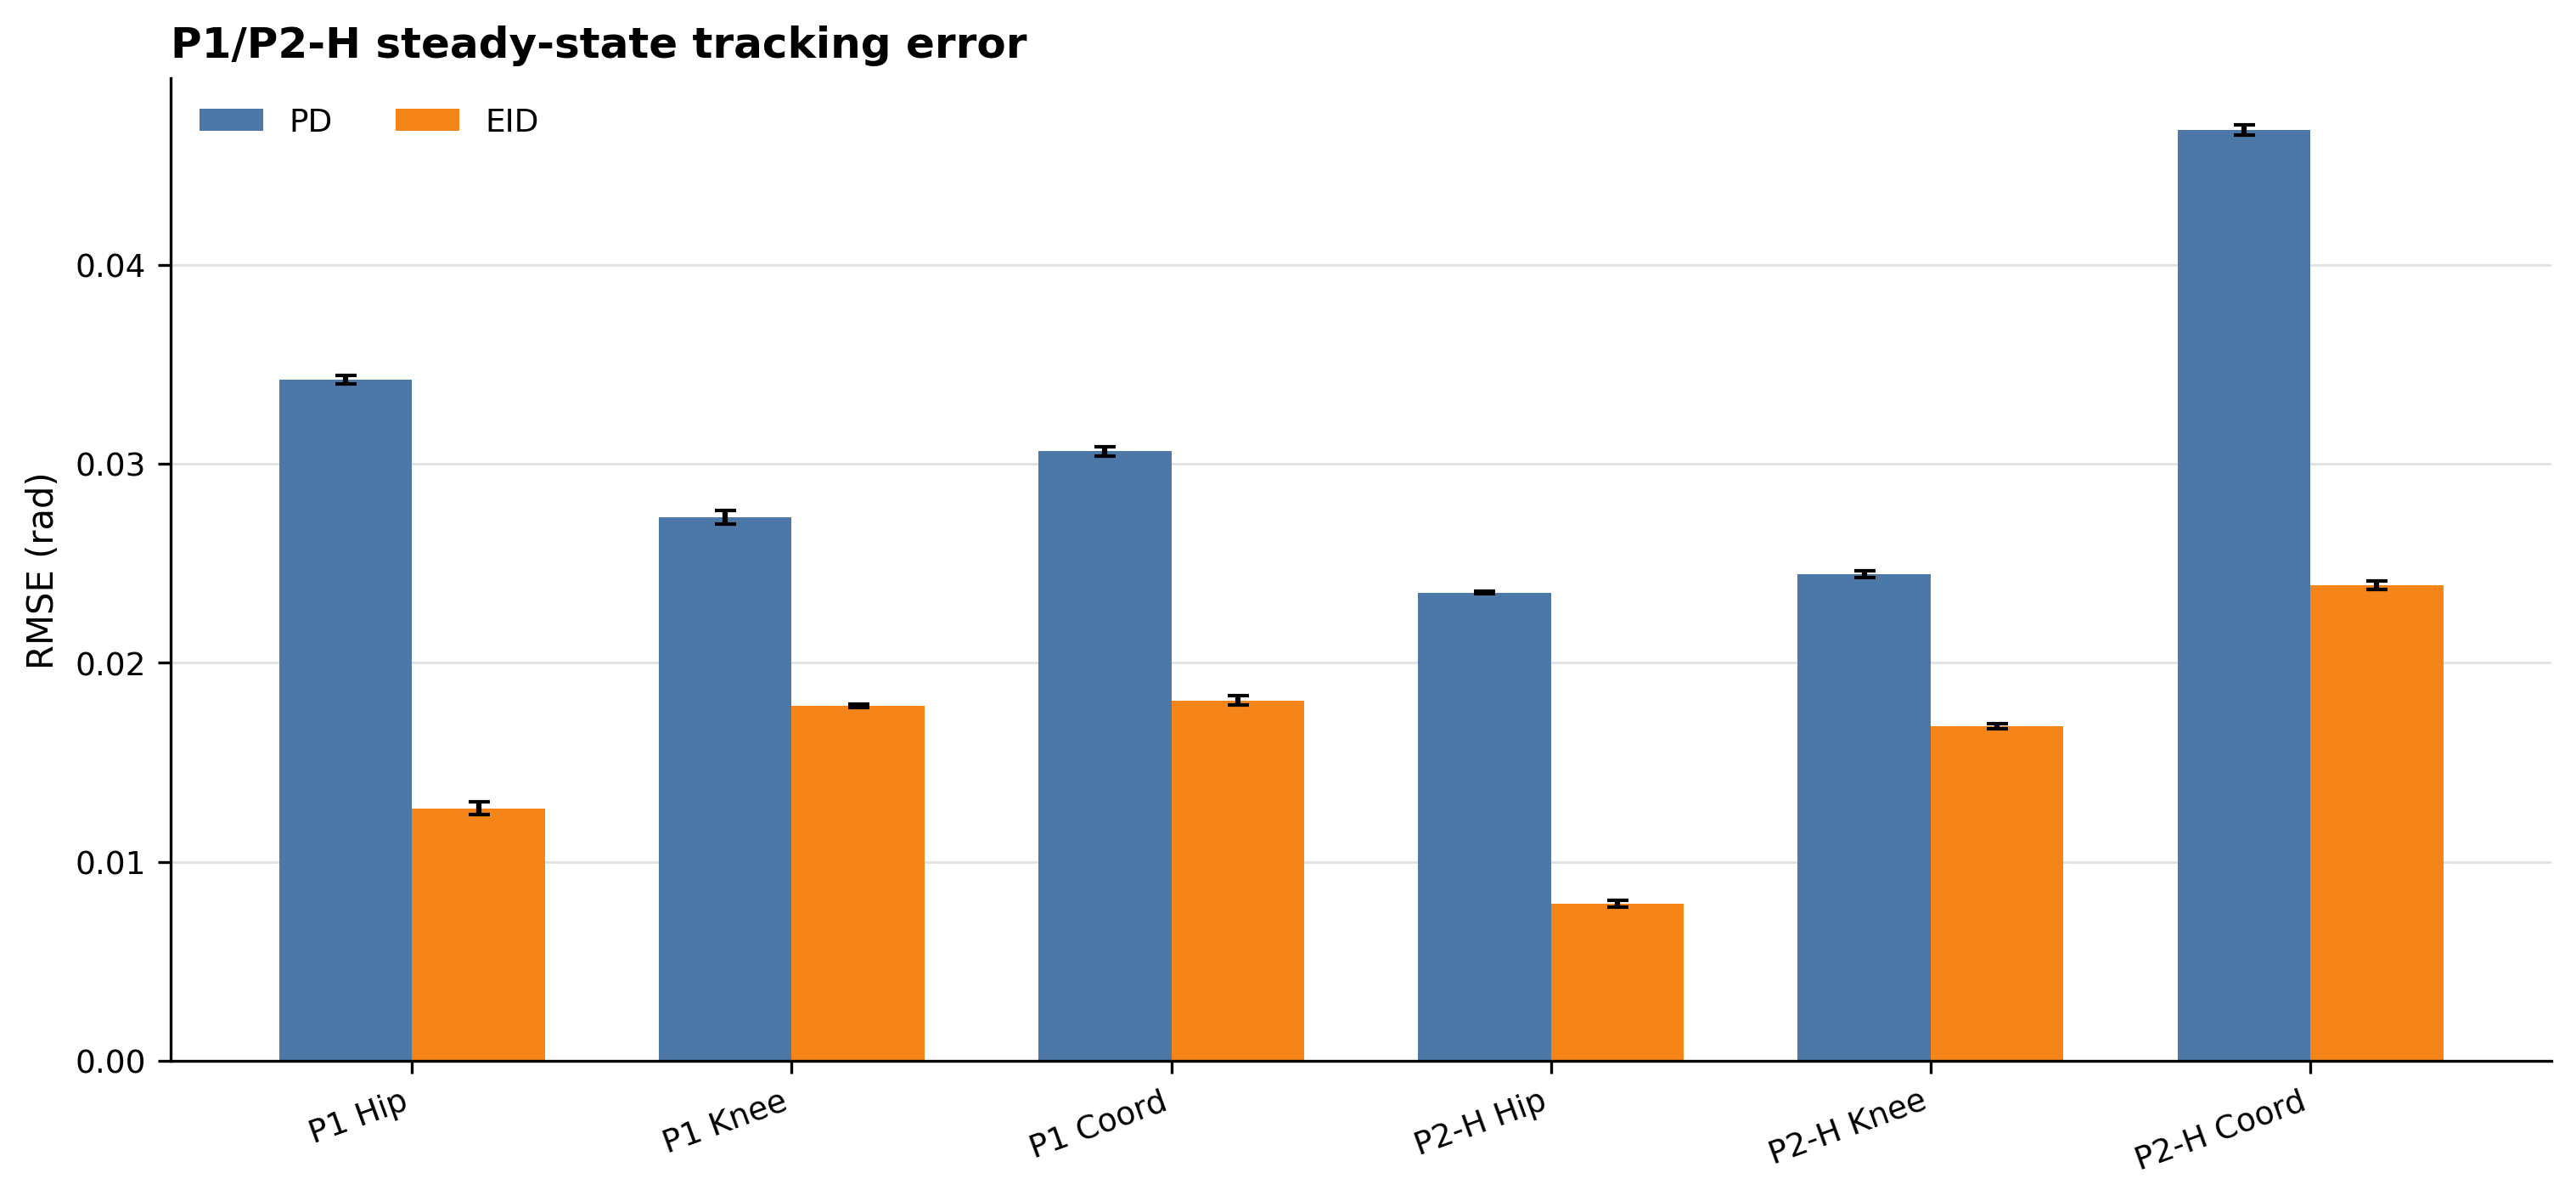
\includegraphics[width=0.92\textwidth]{figures/real_p1_p2_tracking_summary.png}
\caption{P1 无扰动与 P2-H 髋人工扰动实验的稳态 RMSE 对比。EID 整体结构在两个实验中均降低髋、膝和协调误差。}
\end{figure}


\begin{table}[htbp]
\centering
\footnotesize
\caption{P1/P2-H 稳态 RMSE 对比}
\begin{tabularx}{\textwidth}{YYYYY}
\toprule
实验 & 指标 & PD & EID & EID 相对变化 \\
\midrule
P1 & 髋 RMSE rad & 0.0342 & 0.0127 & -62.9\% \\
P1 & 膝 RMSE rad & 0.0273 & 0.0178 & -34.7\% \\
P1 & 协调 RMSE rad & 0.0306 & 0.0181 & -40.9\% \\
P2-H & 髋 RMSE rad & 0.0235 & 0.0079 & -66.4\% \\
P2-H & 膝 RMSE rad & 0.0244 & 0.0168 & -31.2\% \\
P2-H & 协调 RMSE rad & 0.0468 & 0.0239 & -48.9\% \\
\bottomrule
\end{tabularx}
\end{table}


P1 结果支持 EID 整体结构通过无扰动门槛验证：在没有外扰时，EID 整体结构没有引入更大的跟踪误差或协调误差，且各项 RMSE 均低于 PD。P2-H 的全稳态统计也显示 EID 的误差低于 PD，说明在髋人工扰动实验中，EID 整体结构没有使非受扰膝关节误差增加。

但是，P2-H 不能直接写成严格的扰动窗口抗扰结论。由于人工推的开始/结束时间没有进入日志，本轮只能报告全稳态段指标，不能计算受扰窗口 RMSE、峰值误差或恢复时间。

因此，P1 可作为无扰动门槛验证；P2-H 只能作为人工扰动工况下的全稳态统计结果，不能作为严格扰动窗口抗扰结论。

\begin{figure}[htbp]
\centering
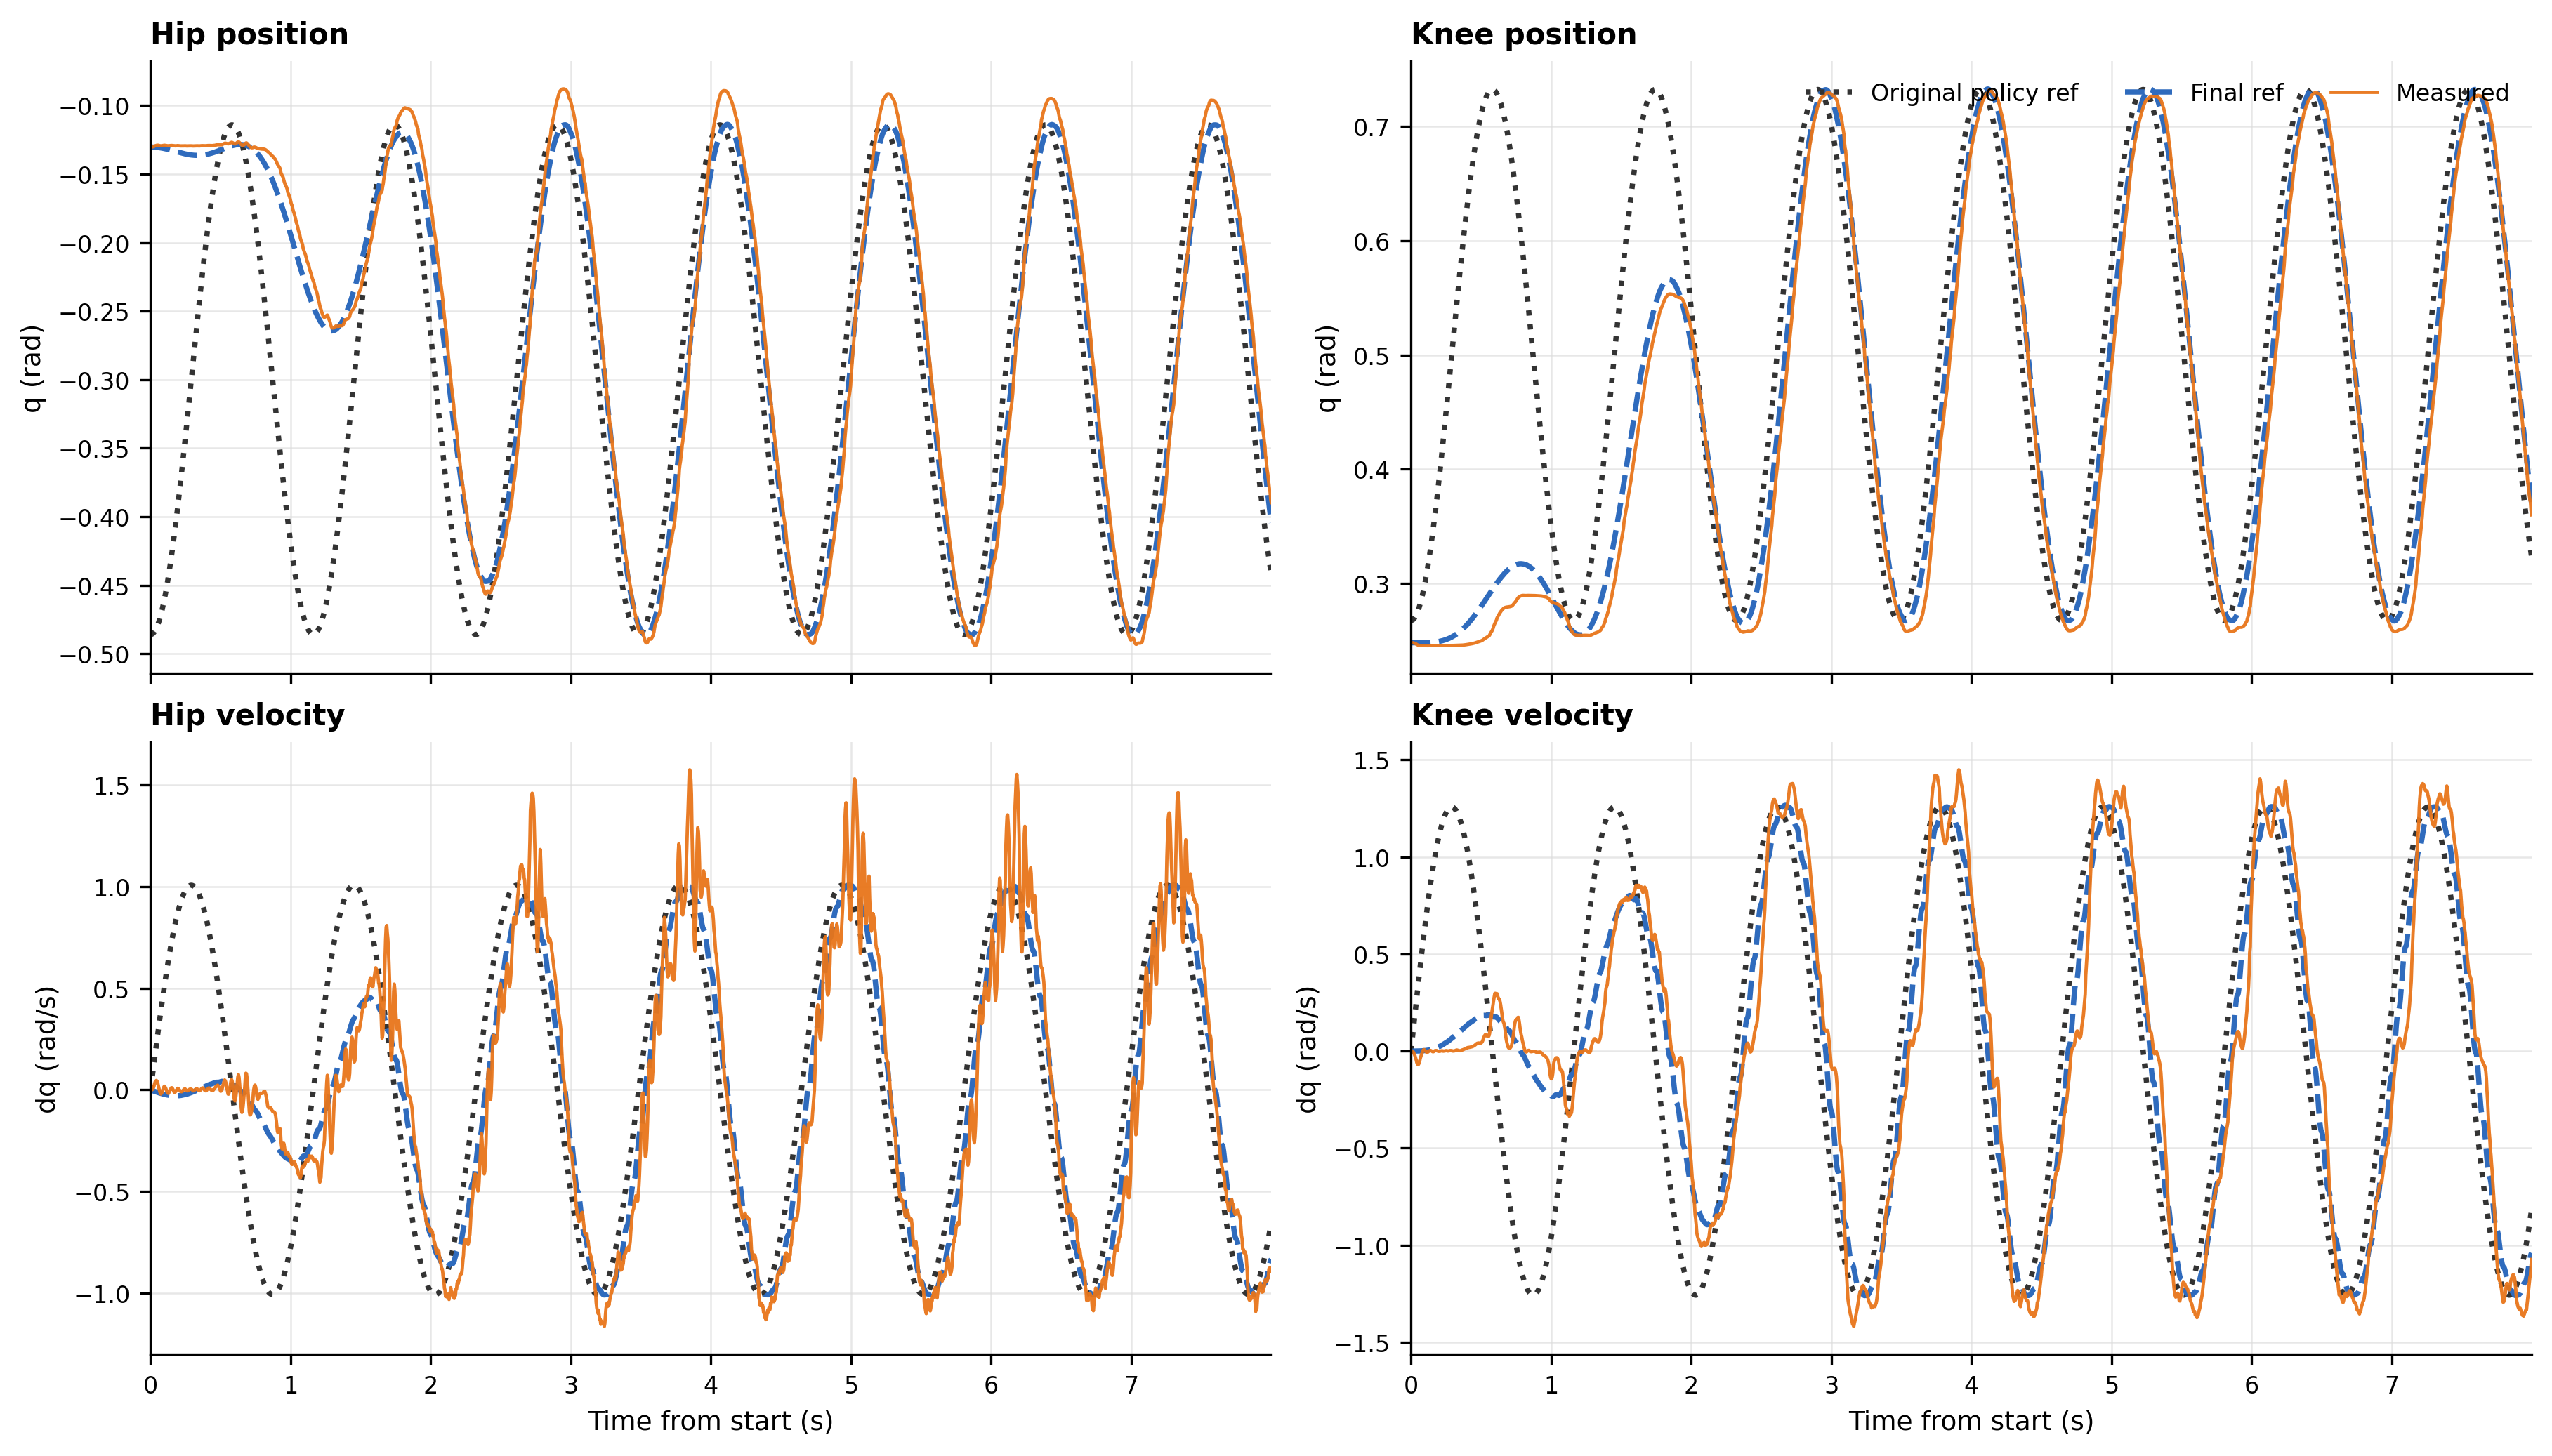
\includegraphics[width=0.92\textwidth]{figures/real_ts_p1_eid_r01.png}
\caption{P1 EID 整体结构代表性时序，重复 r01。位置和速度均从 0 s 开始绘制，可见启动混入阶段最终参考逐步接入原始策略参考；稳态段中实测状态跟随最终参考。}
\end{figure}


\begin{figure}[htbp]
\centering
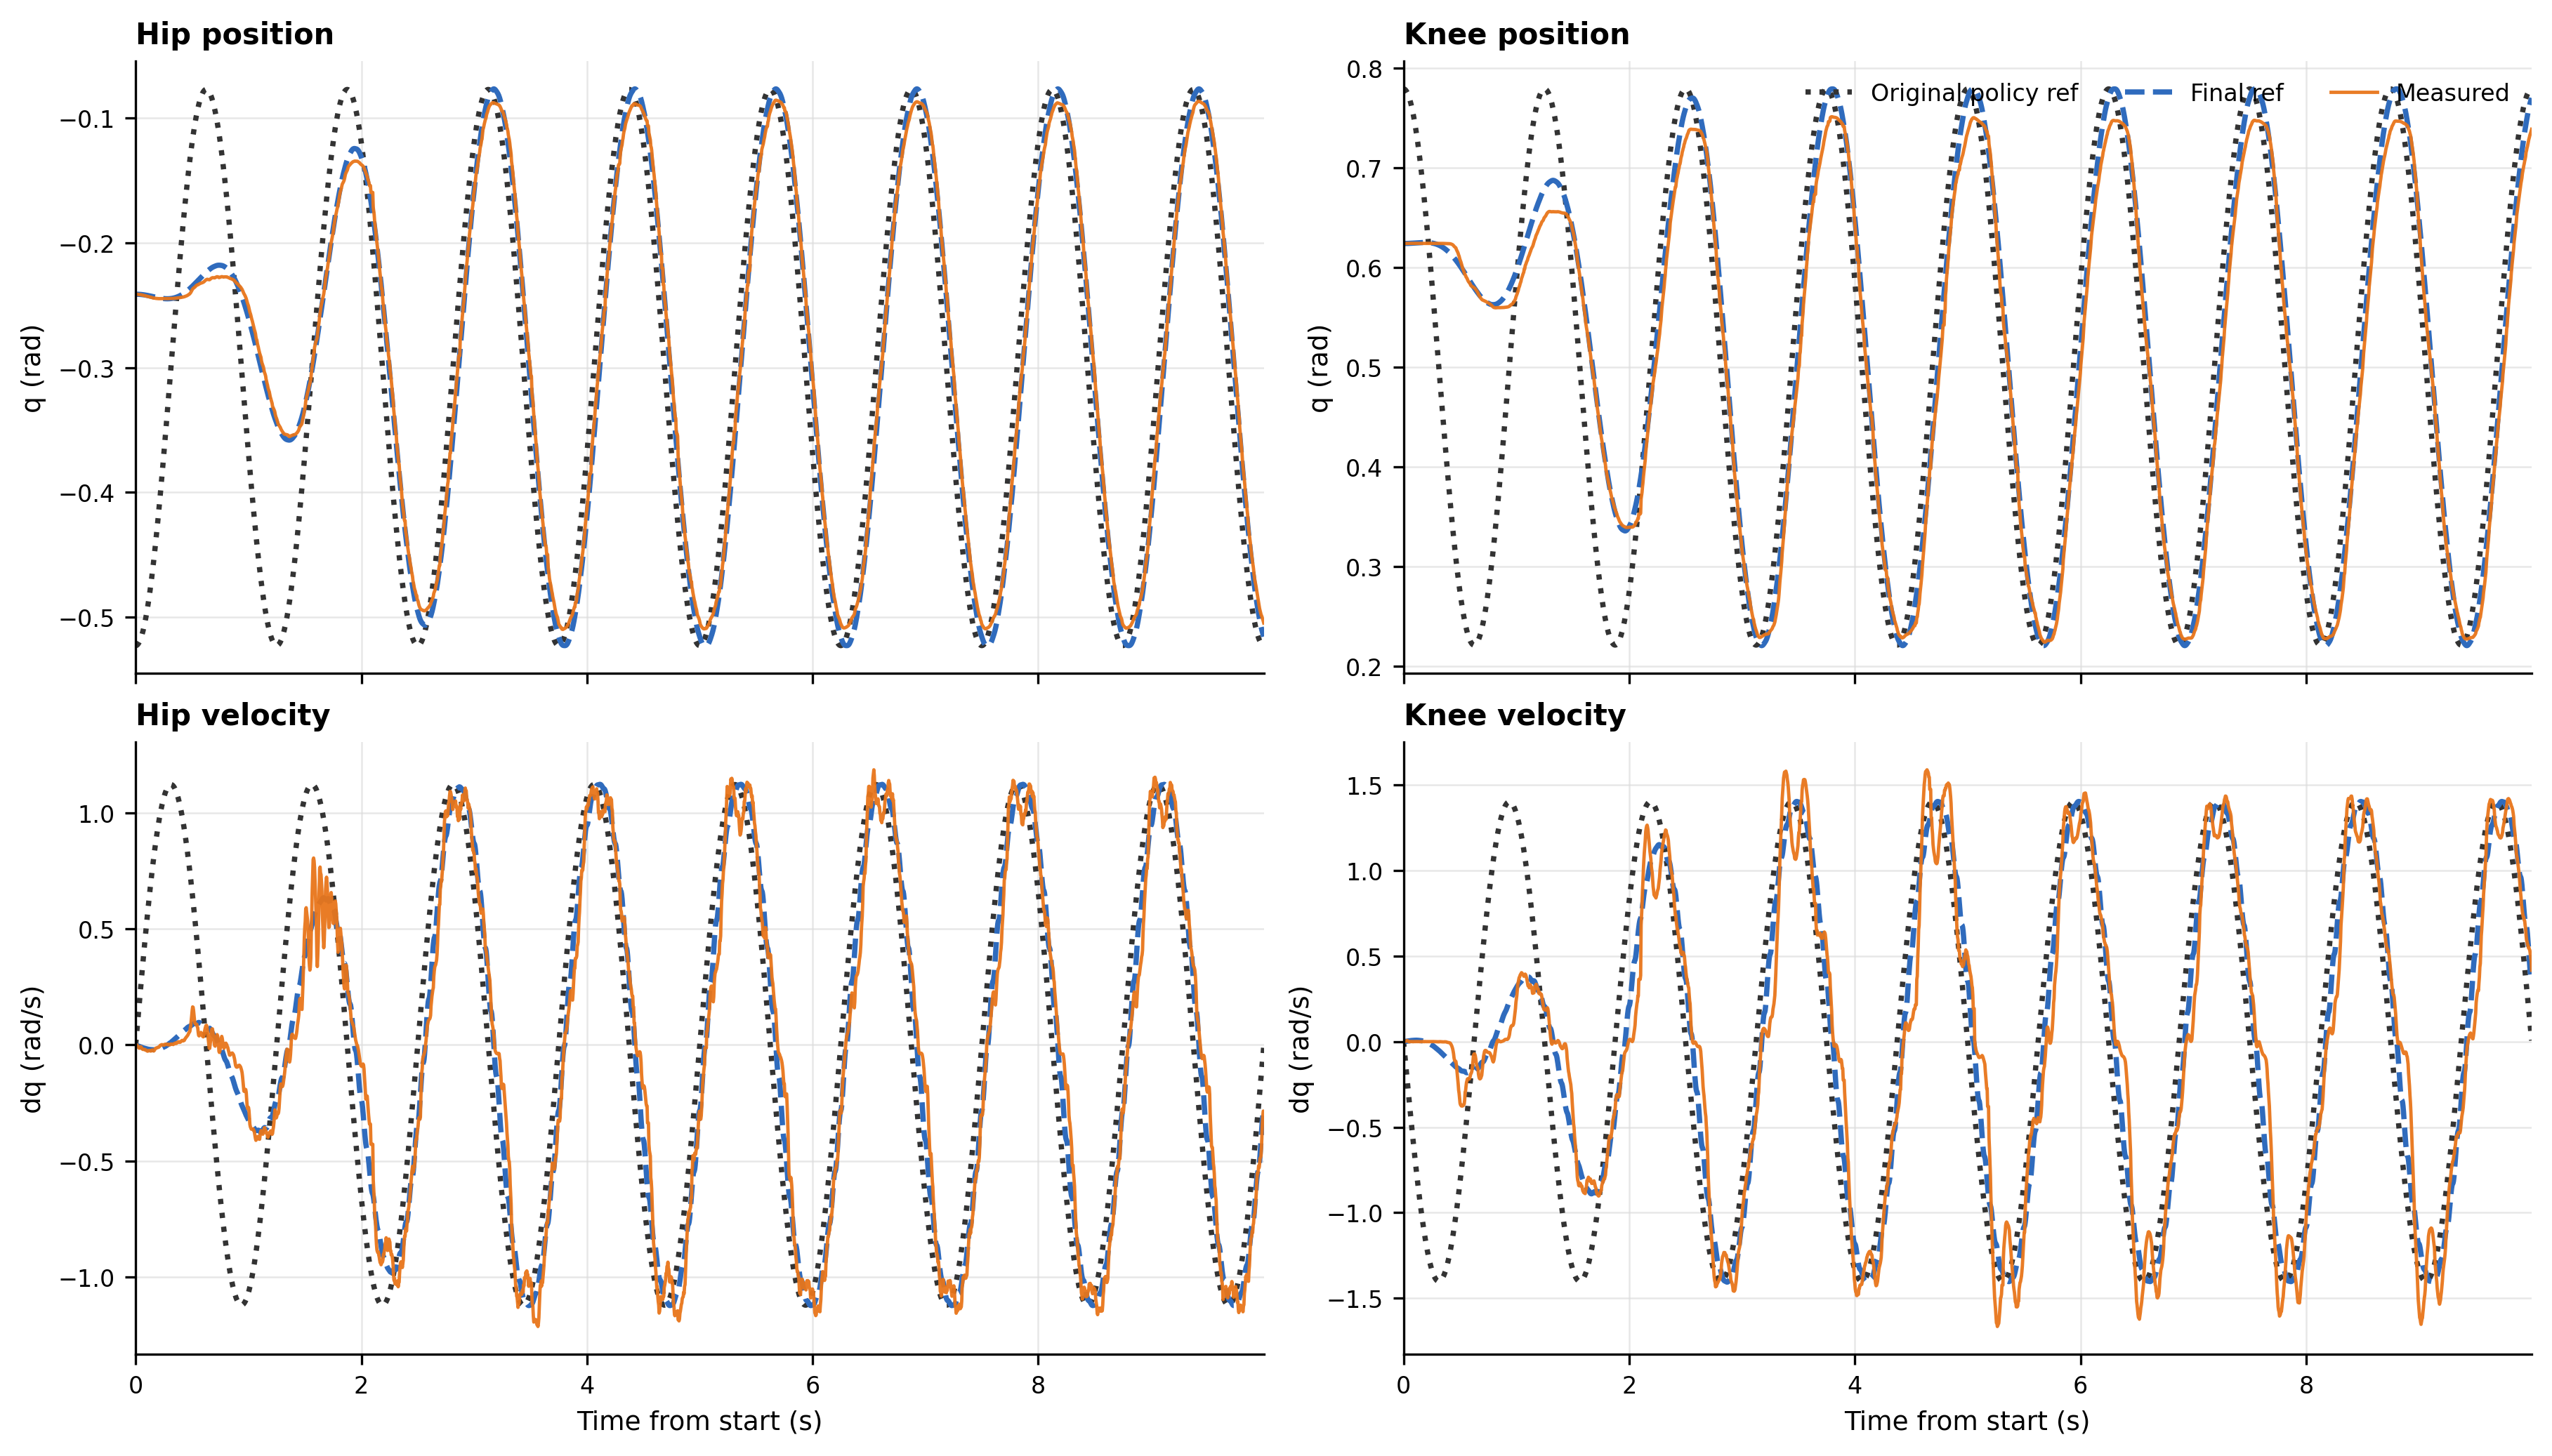
\includegraphics[width=0.92\textwidth]{figures/real_ts_p2h_eid_r01.png}
\caption{P2-H EID 整体结构代表性时序，重复 r01。该图展示髋人工扰动实验中的位置和速度跟踪，但由于人工扰动窗口未记录，图中不标注扰动区间。}
\end{figure}


\subsection{P1/P2-H：误差收益对应的力矩代价}


\begin{figure}[htbp]
\centering
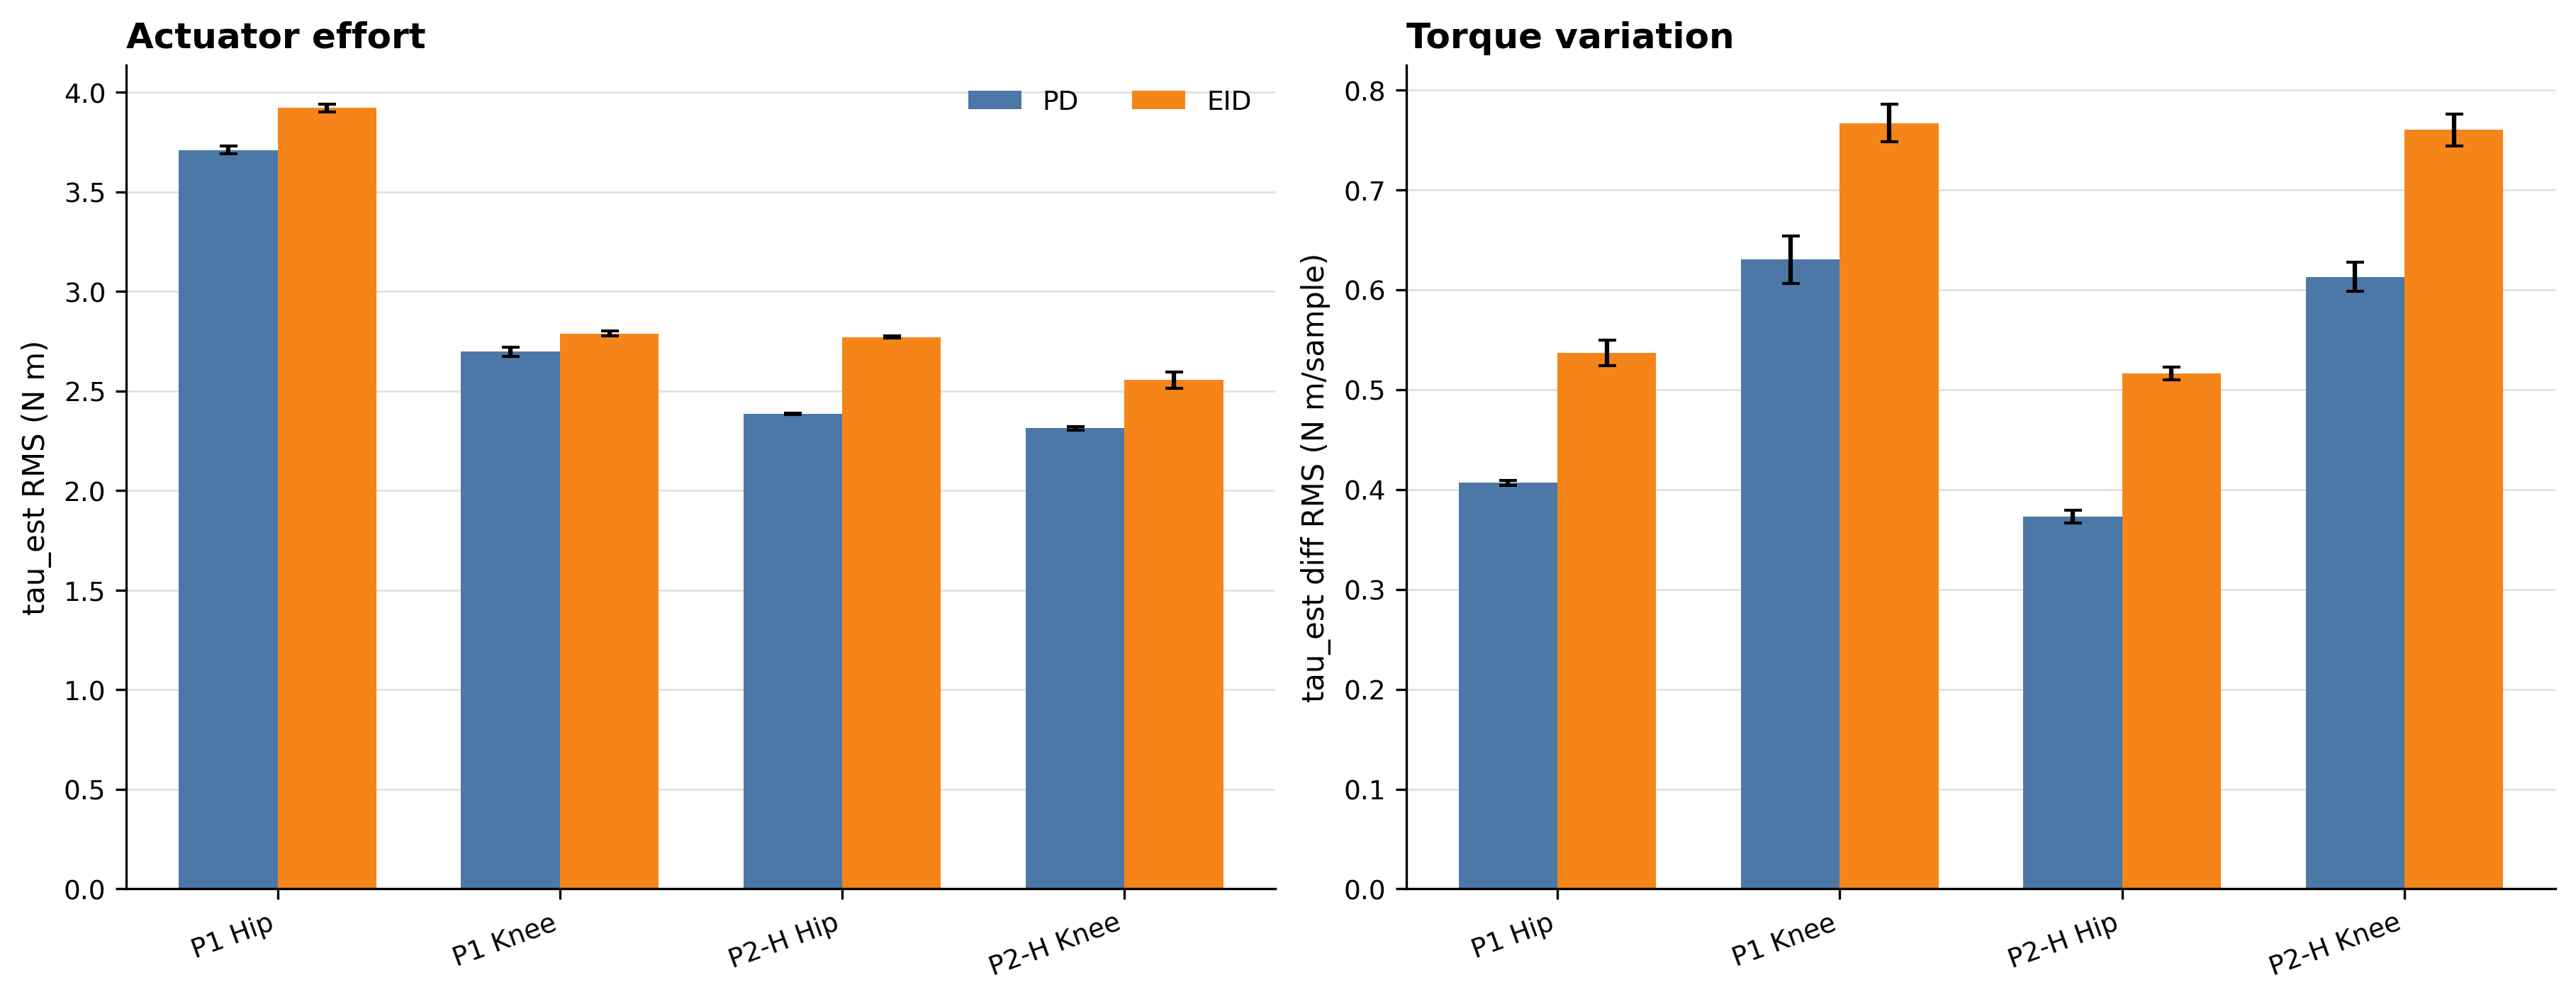
\includegraphics[width=0.92\textwidth]{figures/real_p1_p2_torque_cost.png}
\caption{P1/P2-H 的 $\tau_\mathrm{est}$ RMS 与 $\Delta \tau_\mathrm{est}$ RMS 对比。EID 整体结构的跟踪收益伴随更高的力矩变化量。}
\end{figure}


\begin{table}[htbp]
\centering
\footnotesize
\caption{P1/P2-H 力矩代价对比}
\begin{tabularx}{\textwidth}{YYYYY}
\toprule
实验 & 指标 & PD & EID & EID 相对变化 \\
\midrule
P1 & 髋 $\tau_\mathrm{est}$ RMS N·m & 3.7098 & 3.9202 & +5.7\% \\
P1 & 膝 $\tau_\mathrm{est}$ RMS N·m & 2.6972 & 2.7873 & +3.3\% \\
P1 & 髋 $\Delta \tau_\mathrm{est}$ RMS & 0.4067 & 0.5370 & +32.0\% \\
P1 & 膝 $\Delta \tau_\mathrm{est}$ RMS & 0.6302 & 0.7669 & +21.7\% \\
P2-H & 髋 $\tau_\mathrm{est}$ RMS N·m & 2.3849 & 2.7706 & +16.2\% \\
P2-H & 膝 $\tau_\mathrm{est}$ RMS N·m & 2.3128 & 2.5547 & +10.5\% \\
P2-H & 髋 $\Delta \tau_\mathrm{est}$ RMS & 0.3728 & 0.5164 & +38.5\% \\
P2-H & 膝 $\Delta \tau_\mathrm{est}$ RMS & 0.6130 & 0.7603 & +24.0\% \\
\bottomrule
\end{tabularx}
\end{table}


本轮结果表明，EID 整体结构的主要代价不是平均力矩 RMS 大幅上升，而是 $\Delta\tau_\mathrm{est}$ RMS 上升。后续评价不应只看跟踪 RMSE，还应同步报告 $\tau_\mathrm{est}$ RMS、$\Delta\tau_\mathrm{est}$ RMS、$\eta_u$ RMS 和力矩频谱。

\subsection{P2D：双关节软件力矩扰动}


P2D 使用与 P2-H 相同的反相髋膝轨迹，但将扰动改为可复现的软件力矩脉冲。扰动窗口为 $4.0$--$5.4\ \mathrm{s}$，髋关节叠加 $+6\ \mathrm{N\cdot m}$，膝关节叠加 $-4\ \mathrm{N\cdot m}$。P2D 因此可以计算严格的窗口 RMSE、峰值误差和窗口力矩代价。

\begin{figure}[htbp]
\centering
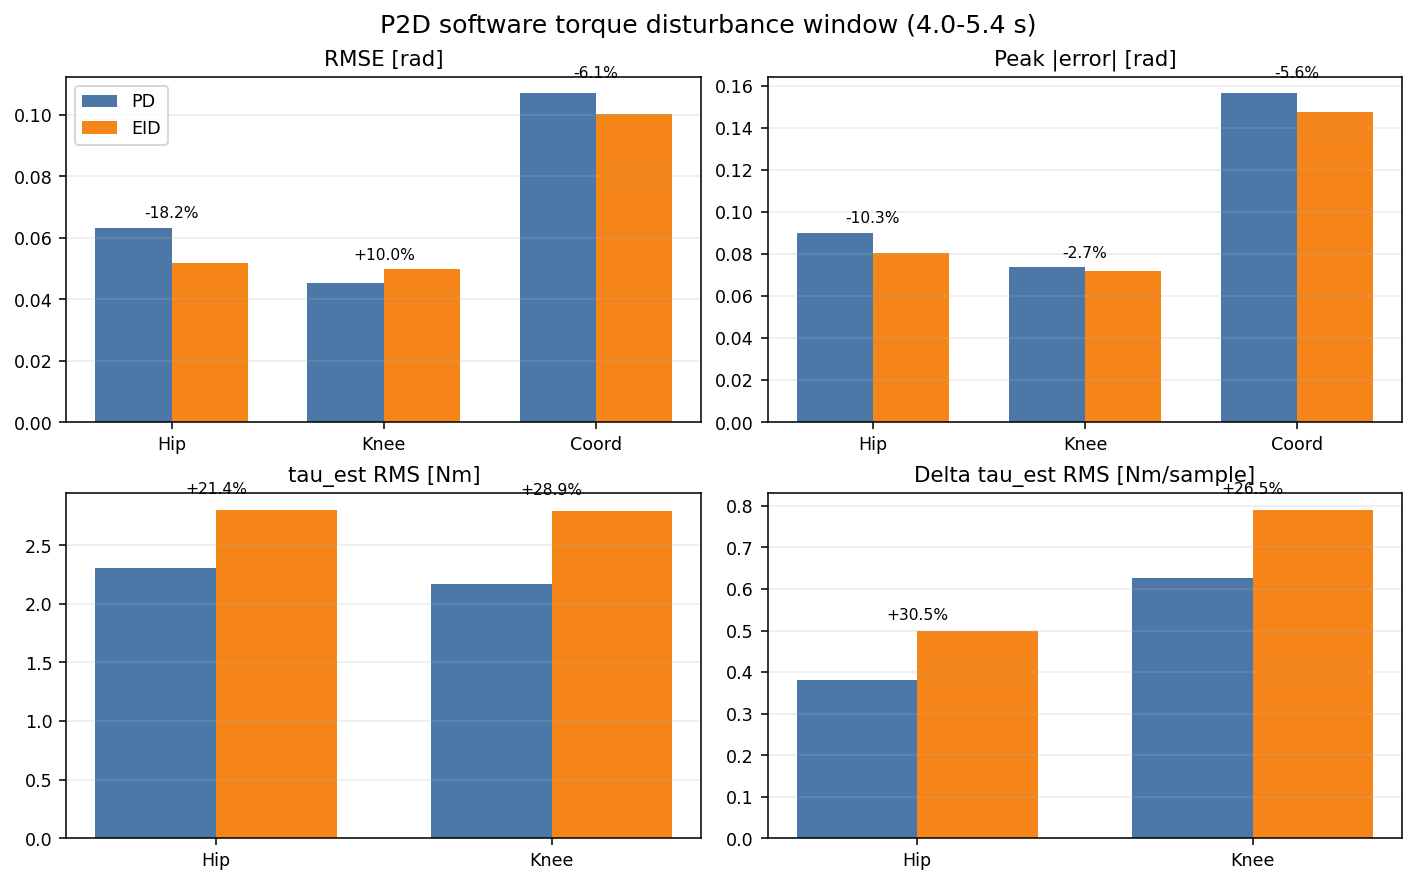
\includegraphics[width=0.92\textwidth]{figures/real_p2d_software_disturbance_summary.png}
\caption{P2D 双关节软件力矩扰动窗口指标。EID 整体结构降低髋窗口 RMSE、协调窗口 RMSE 和峰值误差，但膝窗口 RMSE 略高于 PD，且 $\tau_\mathrm{est}$ RMS 与 $\Delta \tau_\mathrm{est}$ RMS 均上升。}
\end{figure}


\begin{table}[htbp]
\centering
\footnotesize
\caption{P2D 扰动窗口指标}
\begin{tabularx}{\textwidth}{YYYY}
\toprule
指标 & PD & EID & EID 相对变化 \\
\midrule
髋窗口 RMSE rad & 0.0631 & 0.0516 & -18.2\% \\
膝窗口 RMSE rad & 0.0452 & 0.0498 & +10.0\% \\
协调窗口 RMSE rad & 0.1069 & 0.1004 & -6.1\% \\
髋峰值误差 rad & 0.0898 & 0.0806 & -10.3\% \\
膝峰值误差 rad & 0.0738 & 0.0718 & -2.7\% \\
协调峰值误差 rad & 0.1563 & 0.1475 & -5.6\% \\
髋 $\tau_\mathrm{est}$ RMS N·m & 2.3096 & 2.8035 & +21.4\% \\
膝 $\tau_\mathrm{est}$ RMS N·m & 2.1675 & 2.7948 & +28.9\% \\
髋 $\Delta \tau_\mathrm{est}$ RMS & 0.3816 & 0.4979 & +30.5\% \\
膝 $\Delta \tau_\mathrm{est}$ RMS & 0.6254 & 0.7909 & +26.5\% \\
\bottomrule
\end{tabularx}
\end{table}


P2D 的结论比 P2-H 更严格，因为扰动窗口和幅值进入了日志。EID 整体结构在双关节软件扰动下降低了髋关节窗口误差和协调误差，但下降幅度小于 P1/P2-H 的全稳态统计；膝关节窗口 RMSE 略有上升。这说明当前整体结构对软件等效负载的收益主要体现在髋通道和协调峰值抑制，不能概括为所有窗口指标均低于 PD。

\textbf{P2D 小结。} P2D 支持的结论是：在当前 $[+6,-4]\ \mathrm{N\cdot m}$ 软件输入端等效扰动下，EID 整体结构改善髋关节窗口 RMSE、协调窗口 RMSE 和峰值误差，但没有改善膝窗口 RMSE，并且增加力矩 RMS 与力矩变化量。因此，P2D 不能概括为“EID 所有扰动指标均优于 PD”，更准确的表述是“EID 在输入端等效扰动下表现出部分抗扰收益，同时伴随明确力矩代价”。

\begin{figure}[htbp]
\centering
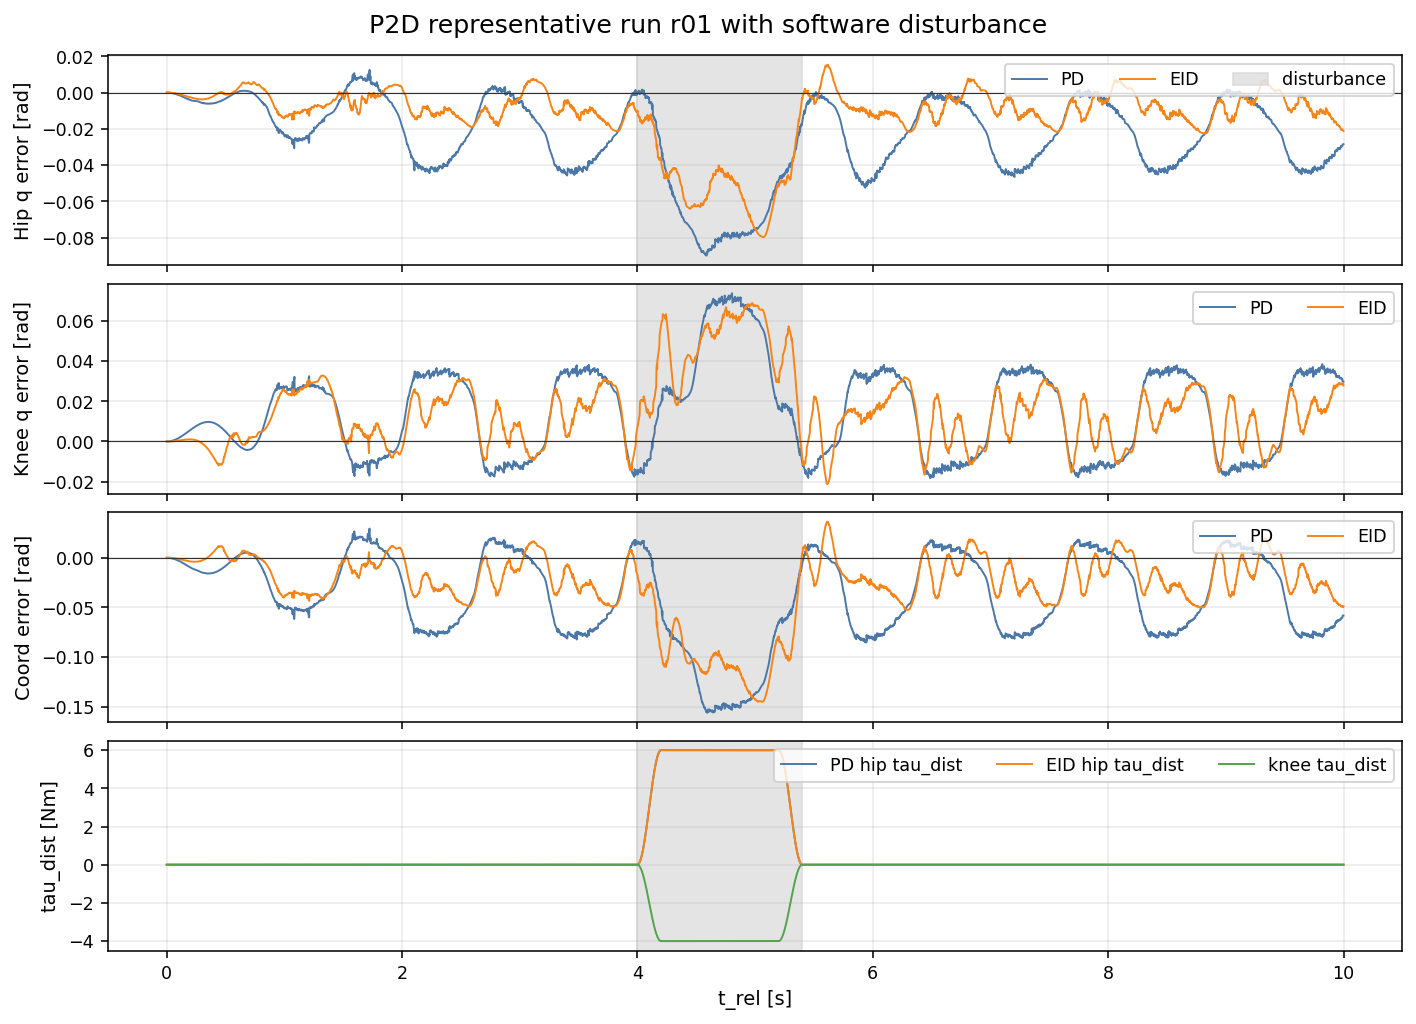
\includegraphics[width=0.92\textwidth]{figures/real_ts_p2d_pd_eid_r01.png}
\caption{P2D 代表性时序，重复 r01。灰色区域为 $4.0$--$5.4\ \mathrm{s}$ 软件扰动窗口。EID 整体结构在髋误差和协调误差峰值上低于 PD，但膝误差曲线在扰动窗口内与 PD 接近。}
\end{figure}


P2D 同时给出了力矩代价：EID 整体结构的 $\tau_\mathrm{est}$ RMS 和 $\Delta \tau_\mathrm{est}$ RMS 都高于 PD。因此，带扰动结果需要同时报告误差收益和力矩变化量，而不能只依据 RMSE 评价控制效果。P2D 中 EID 条件的一次重复在扰动结束后未跑满 10 s，但该日志覆盖完整扰动窗口，因此纳入窗口统计；恢复段统计只基于覆盖恢复窗口的日志解释。

\subsection{P3：Preview-MPC 参考生成}


\begin{figure}[htbp]
\centering
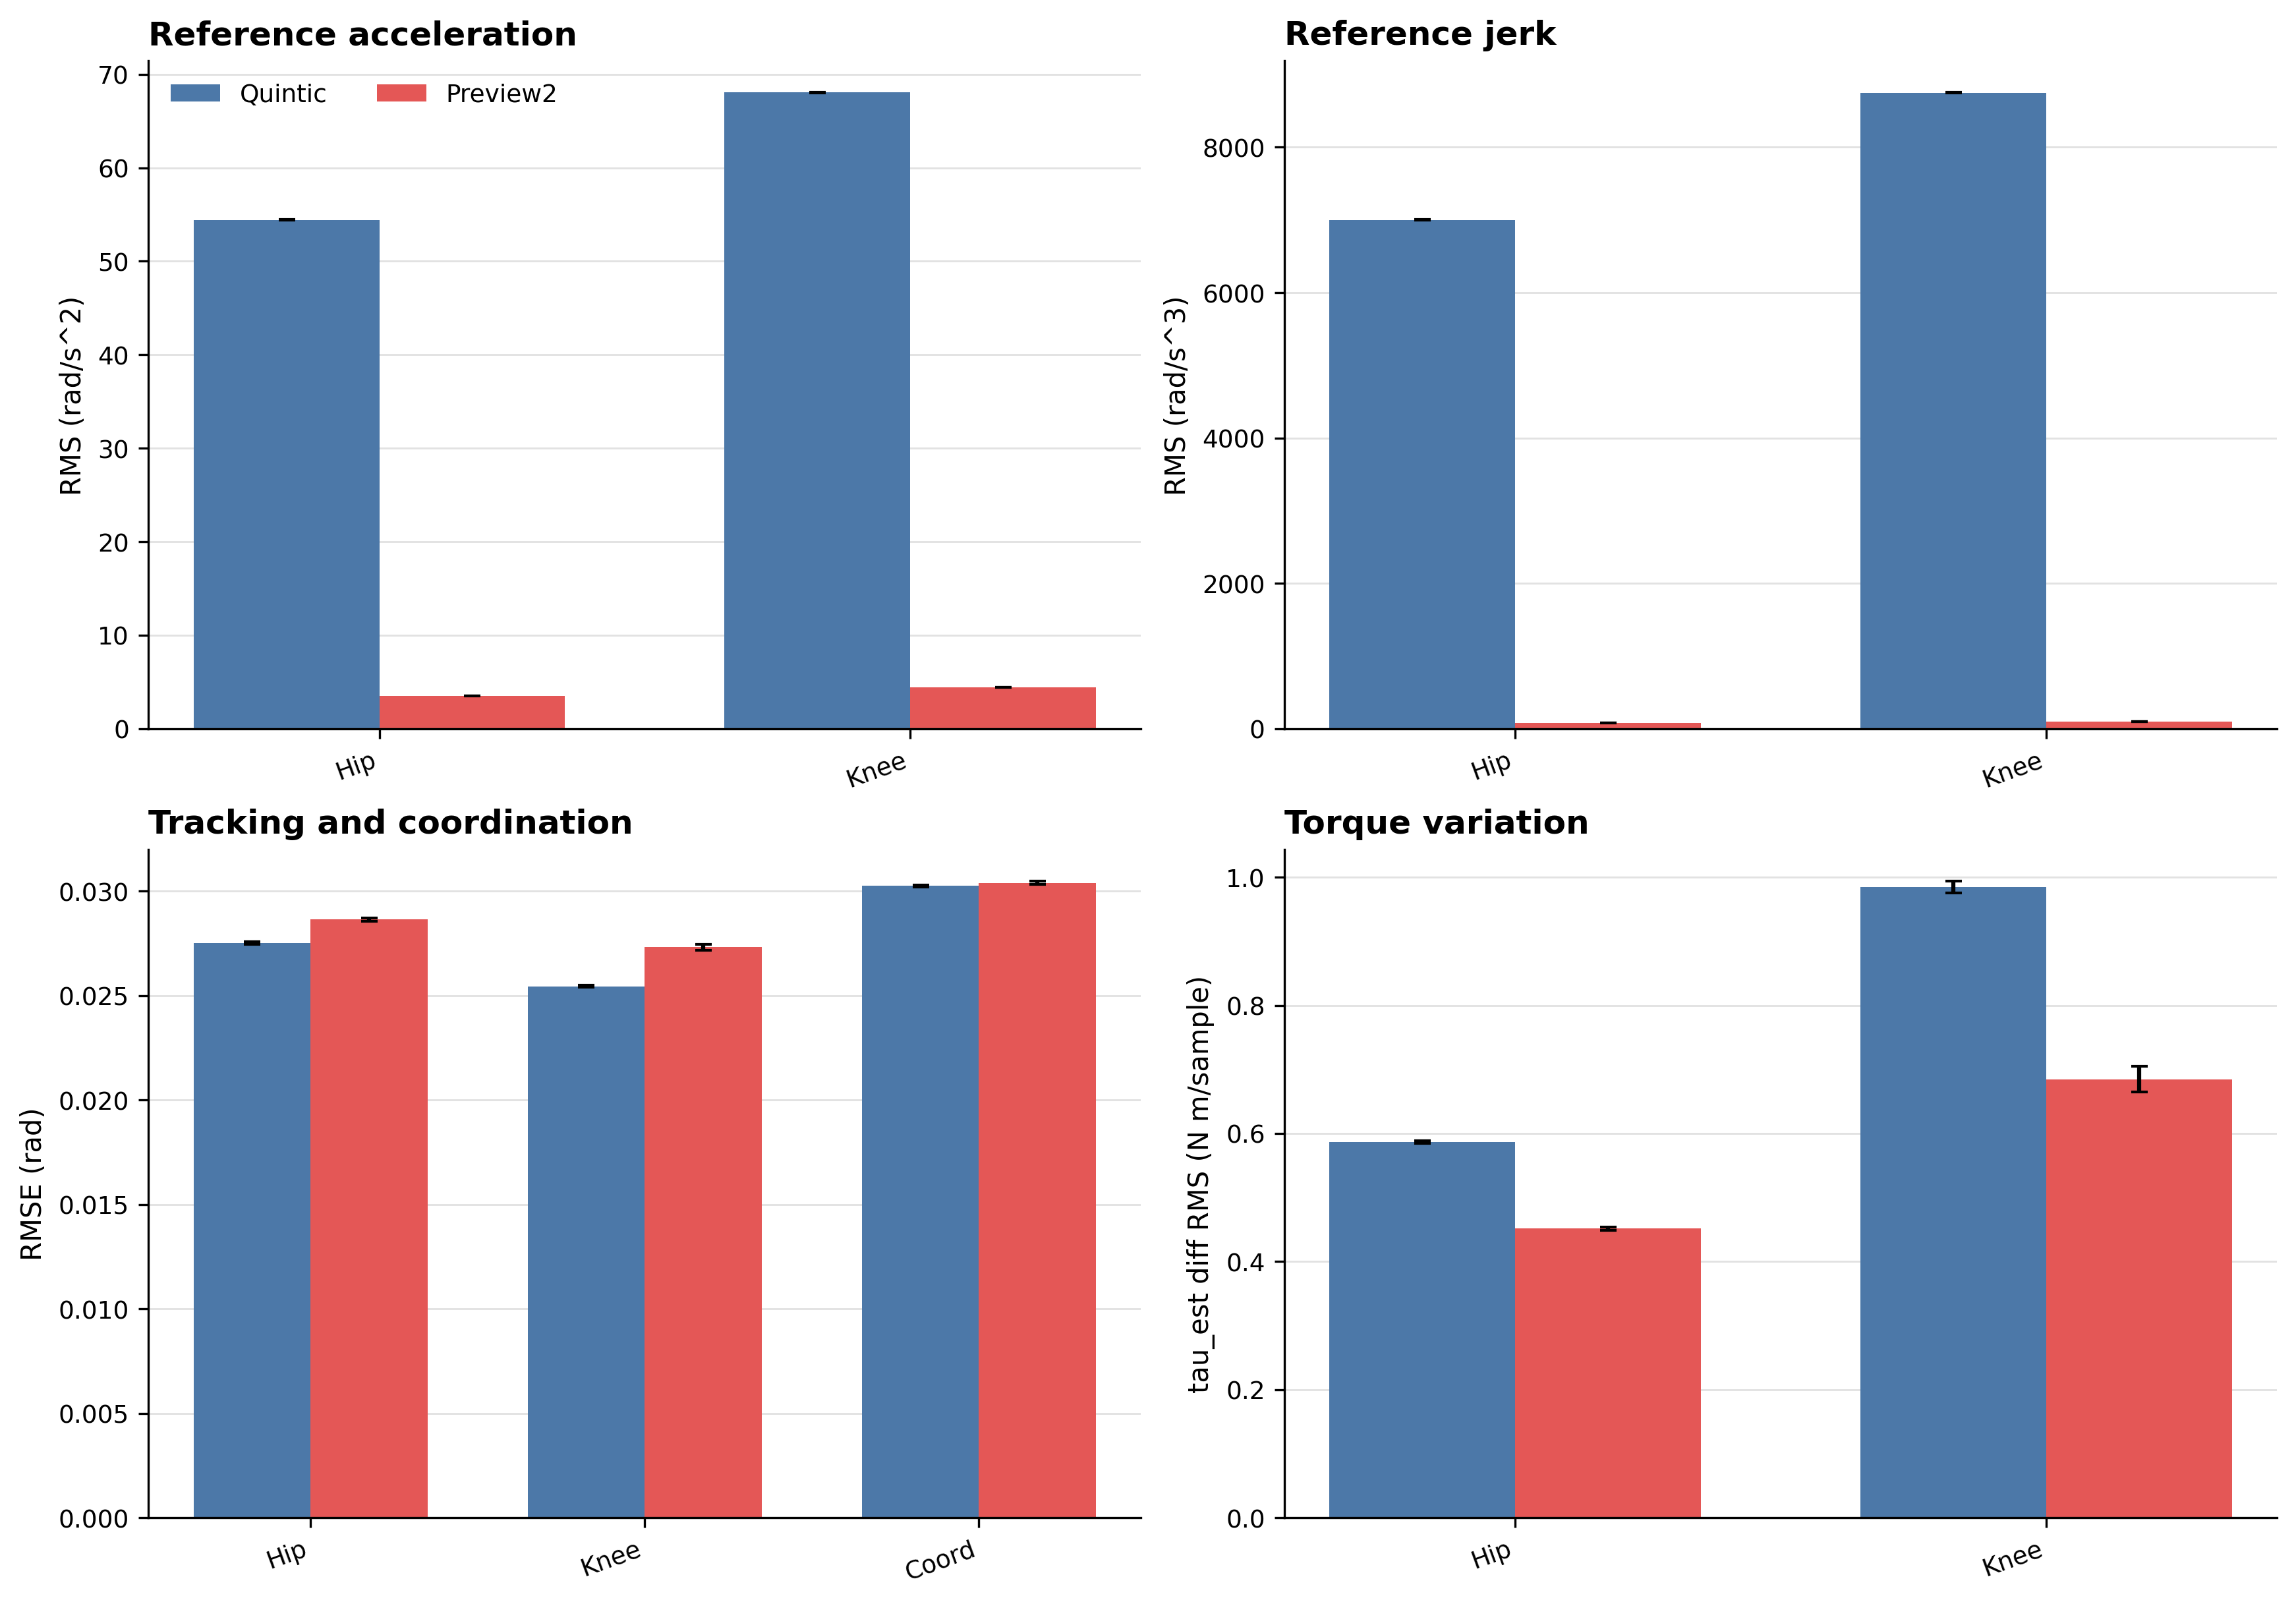
\includegraphics[width=0.92\textwidth]{figures/real_p3_preview_tradeoff.png}
\caption{P3 中零速五次样条与 2 点 Preview-MPC 的参考激励、跟踪误差和力矩变化量对比。Preview-MPC 大幅降低参考高阶激励，并降低力矩变化量。}
\end{figure}


\begin{table}[htbp]
\centering
\footnotesize
\caption{P3 Preview-MPC 指标对比}
\begin{tabularx}{\textwidth}{YYYY}
\toprule
指标 & quintic & preview2 & preview2 相对变化 \\
\midrule
髋参考加速度 RMS rad/s² & 54.4358 & 3.5301 & -93.5\% \\
膝参考加速度 RMS rad/s² & 68.0448 & 4.4126 & -93.5\% \\
髋参考 jerk RMS rad/s³ & 7000.8924 & 80.7808 & -98.8\% \\
膝参考 jerk RMS rad/s³ & 8751.1154 & 100.9760 & -98.8\% \\
髋 RMSE rad & 0.0275 & 0.0286 & +4.1\% \\
膝 RMSE rad & 0.0254 & 0.0273 & +7.4\% \\
协调 RMSE rad & 0.0302 & 0.0304 & +0.5\% \\
髋 $\Delta \tau_\mathrm{est}$ RMS & 0.5866 & 0.4515 & -23.0\% \\
膝 $\Delta \tau_\mathrm{est}$ RMS & 0.9848 & 0.6846 & -30.5\% \\
\bottomrule
\end{tabularx}
\end{table}


Preview-MPC 的主要结果是参考加速度和 jerk 大幅下降，且 $\Delta \tau_\mathrm{est}$ RMS 下降。其代价是髋/膝 RMSE 小幅上升，但协调误差几乎不变。该结果支持将 preview2 作为降低参考尖峰和力矩粗糙度的参考生成候选。

\begin{figure}[htbp]
\centering
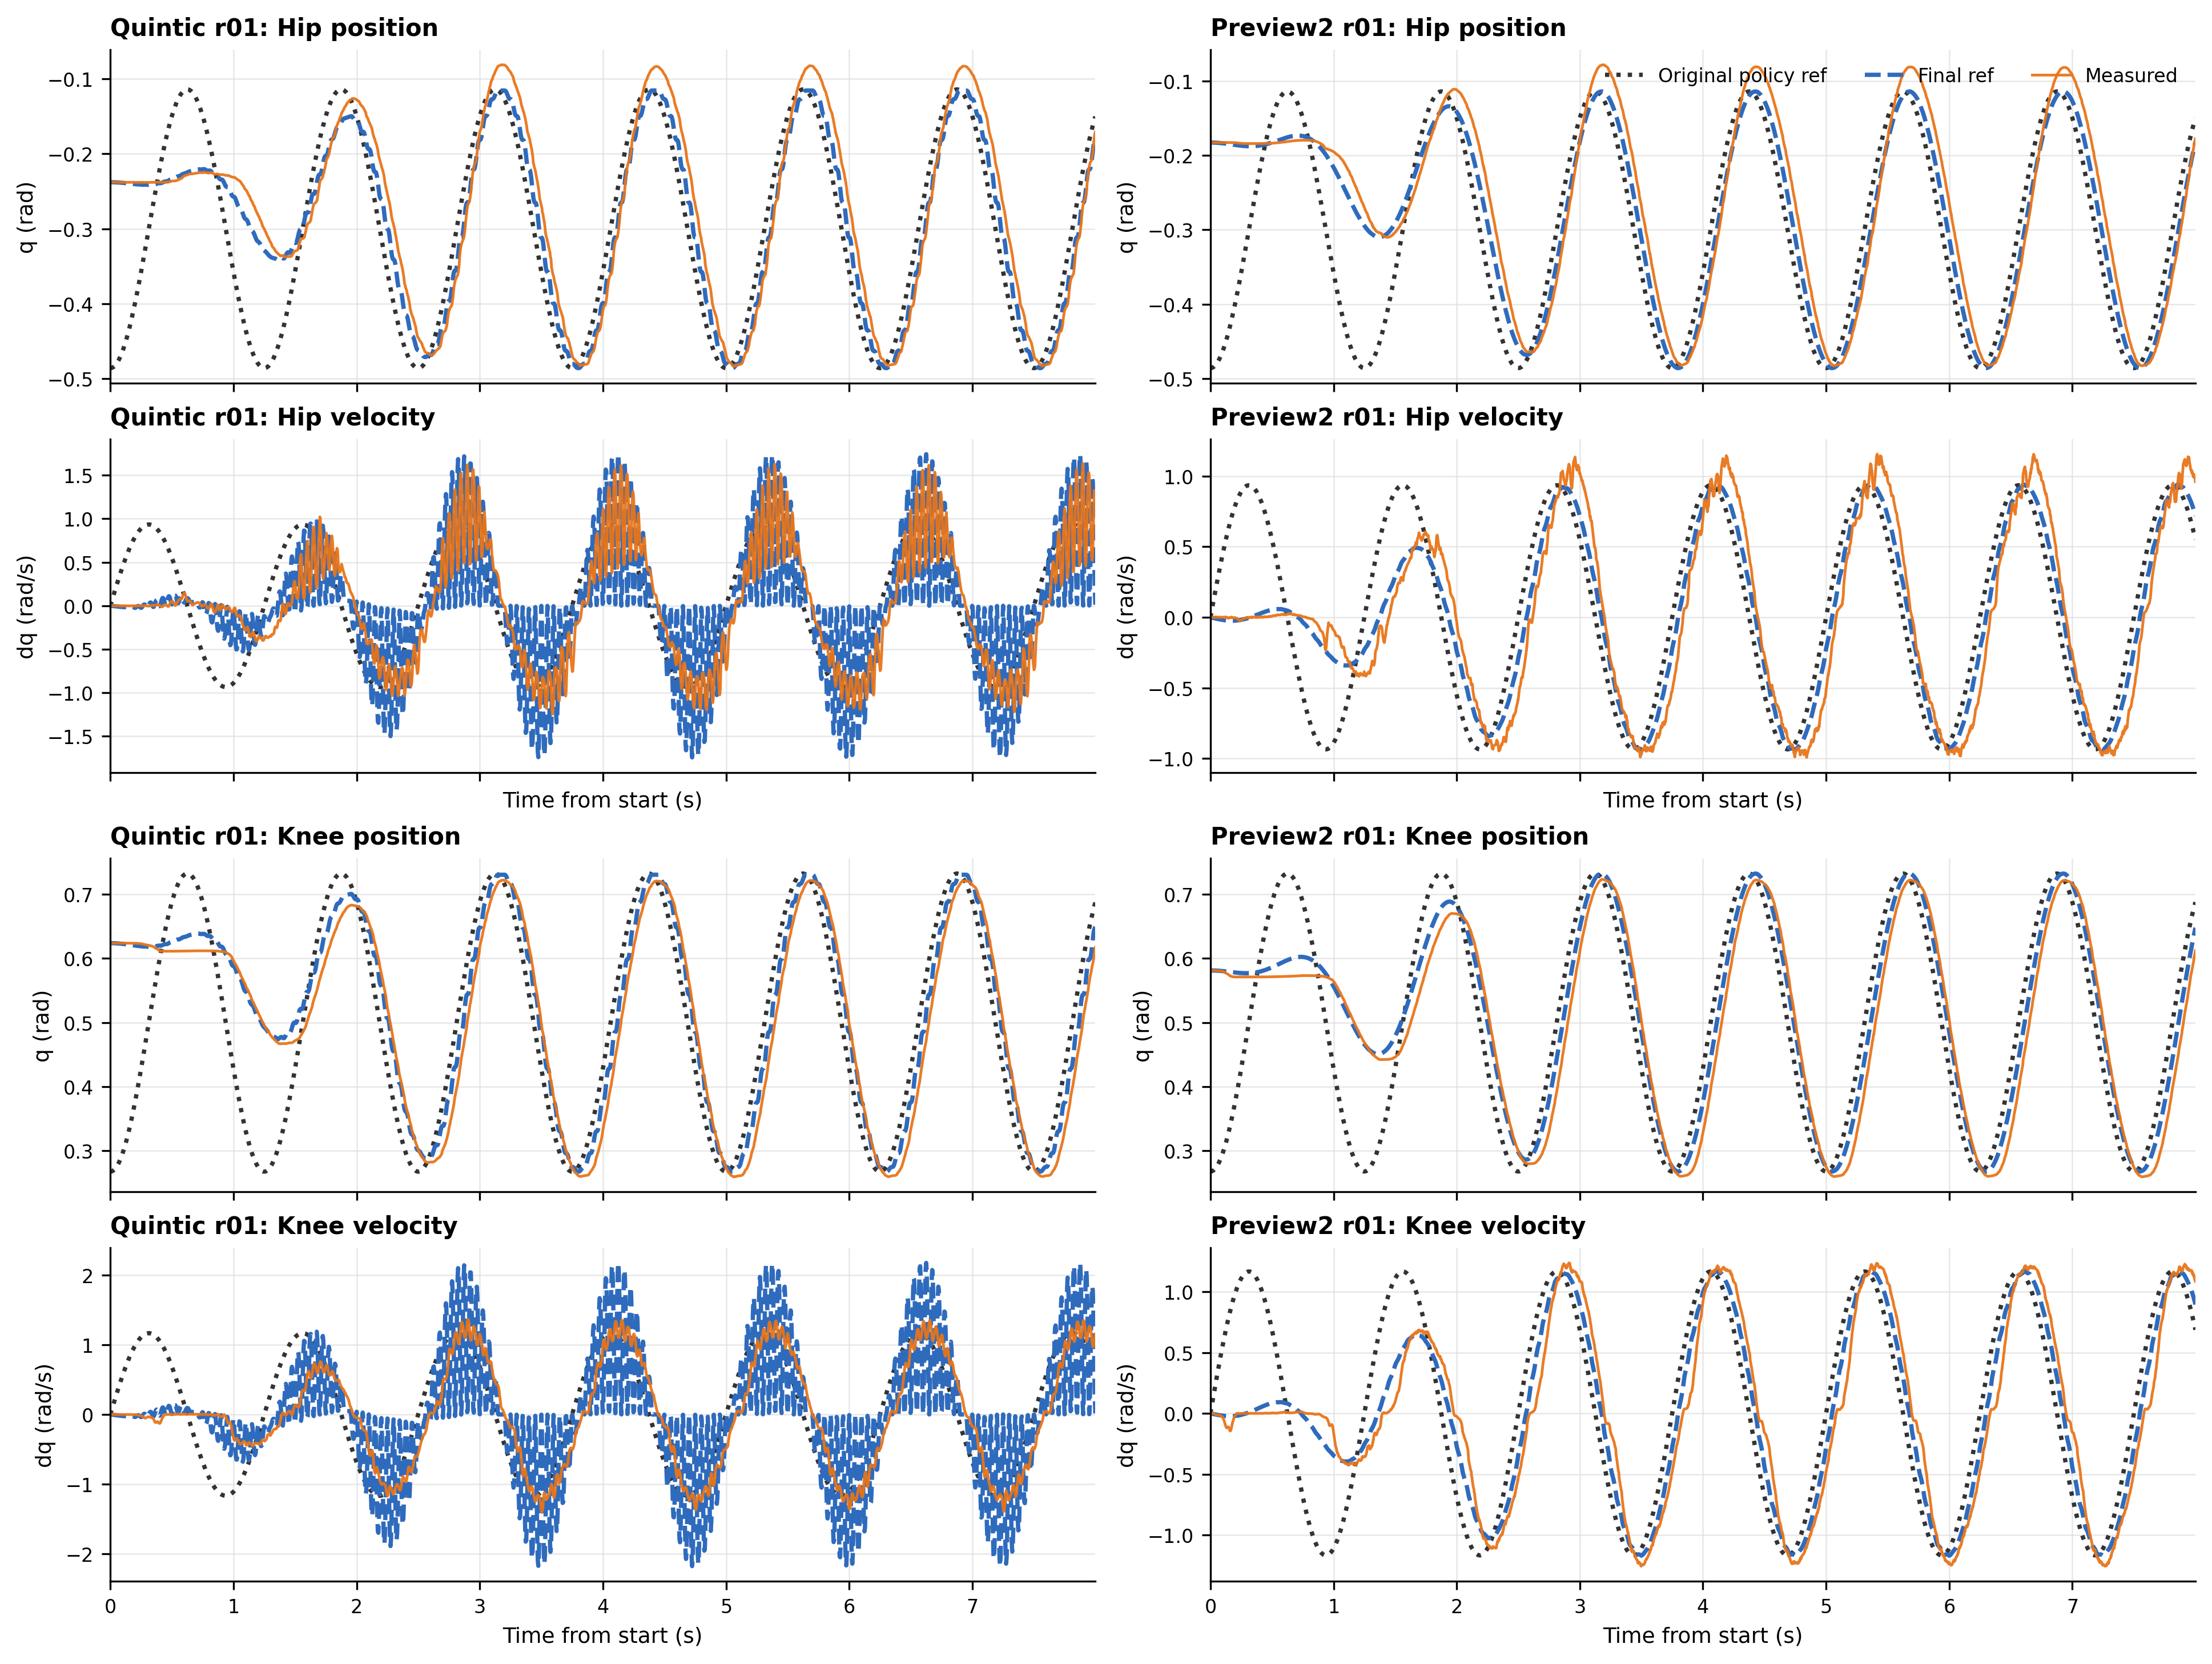
\includegraphics[width=0.92\textwidth]{figures/real_ts_p3_quintic_preview_r01.png}
\caption{P3 代表性时序，重复 r01。左列为零速五次样条，右列为 2 点 Preview-MPC。Preview-MPC 的速度参考明显更平滑，与图 8 中参考加速度和 jerk 降低的统计结果一致。}
\end{figure}


\subsection{P4：$K_o$ 与 $K_u$ 无扰动扫描}


\begin{figure}[htbp]
\centering
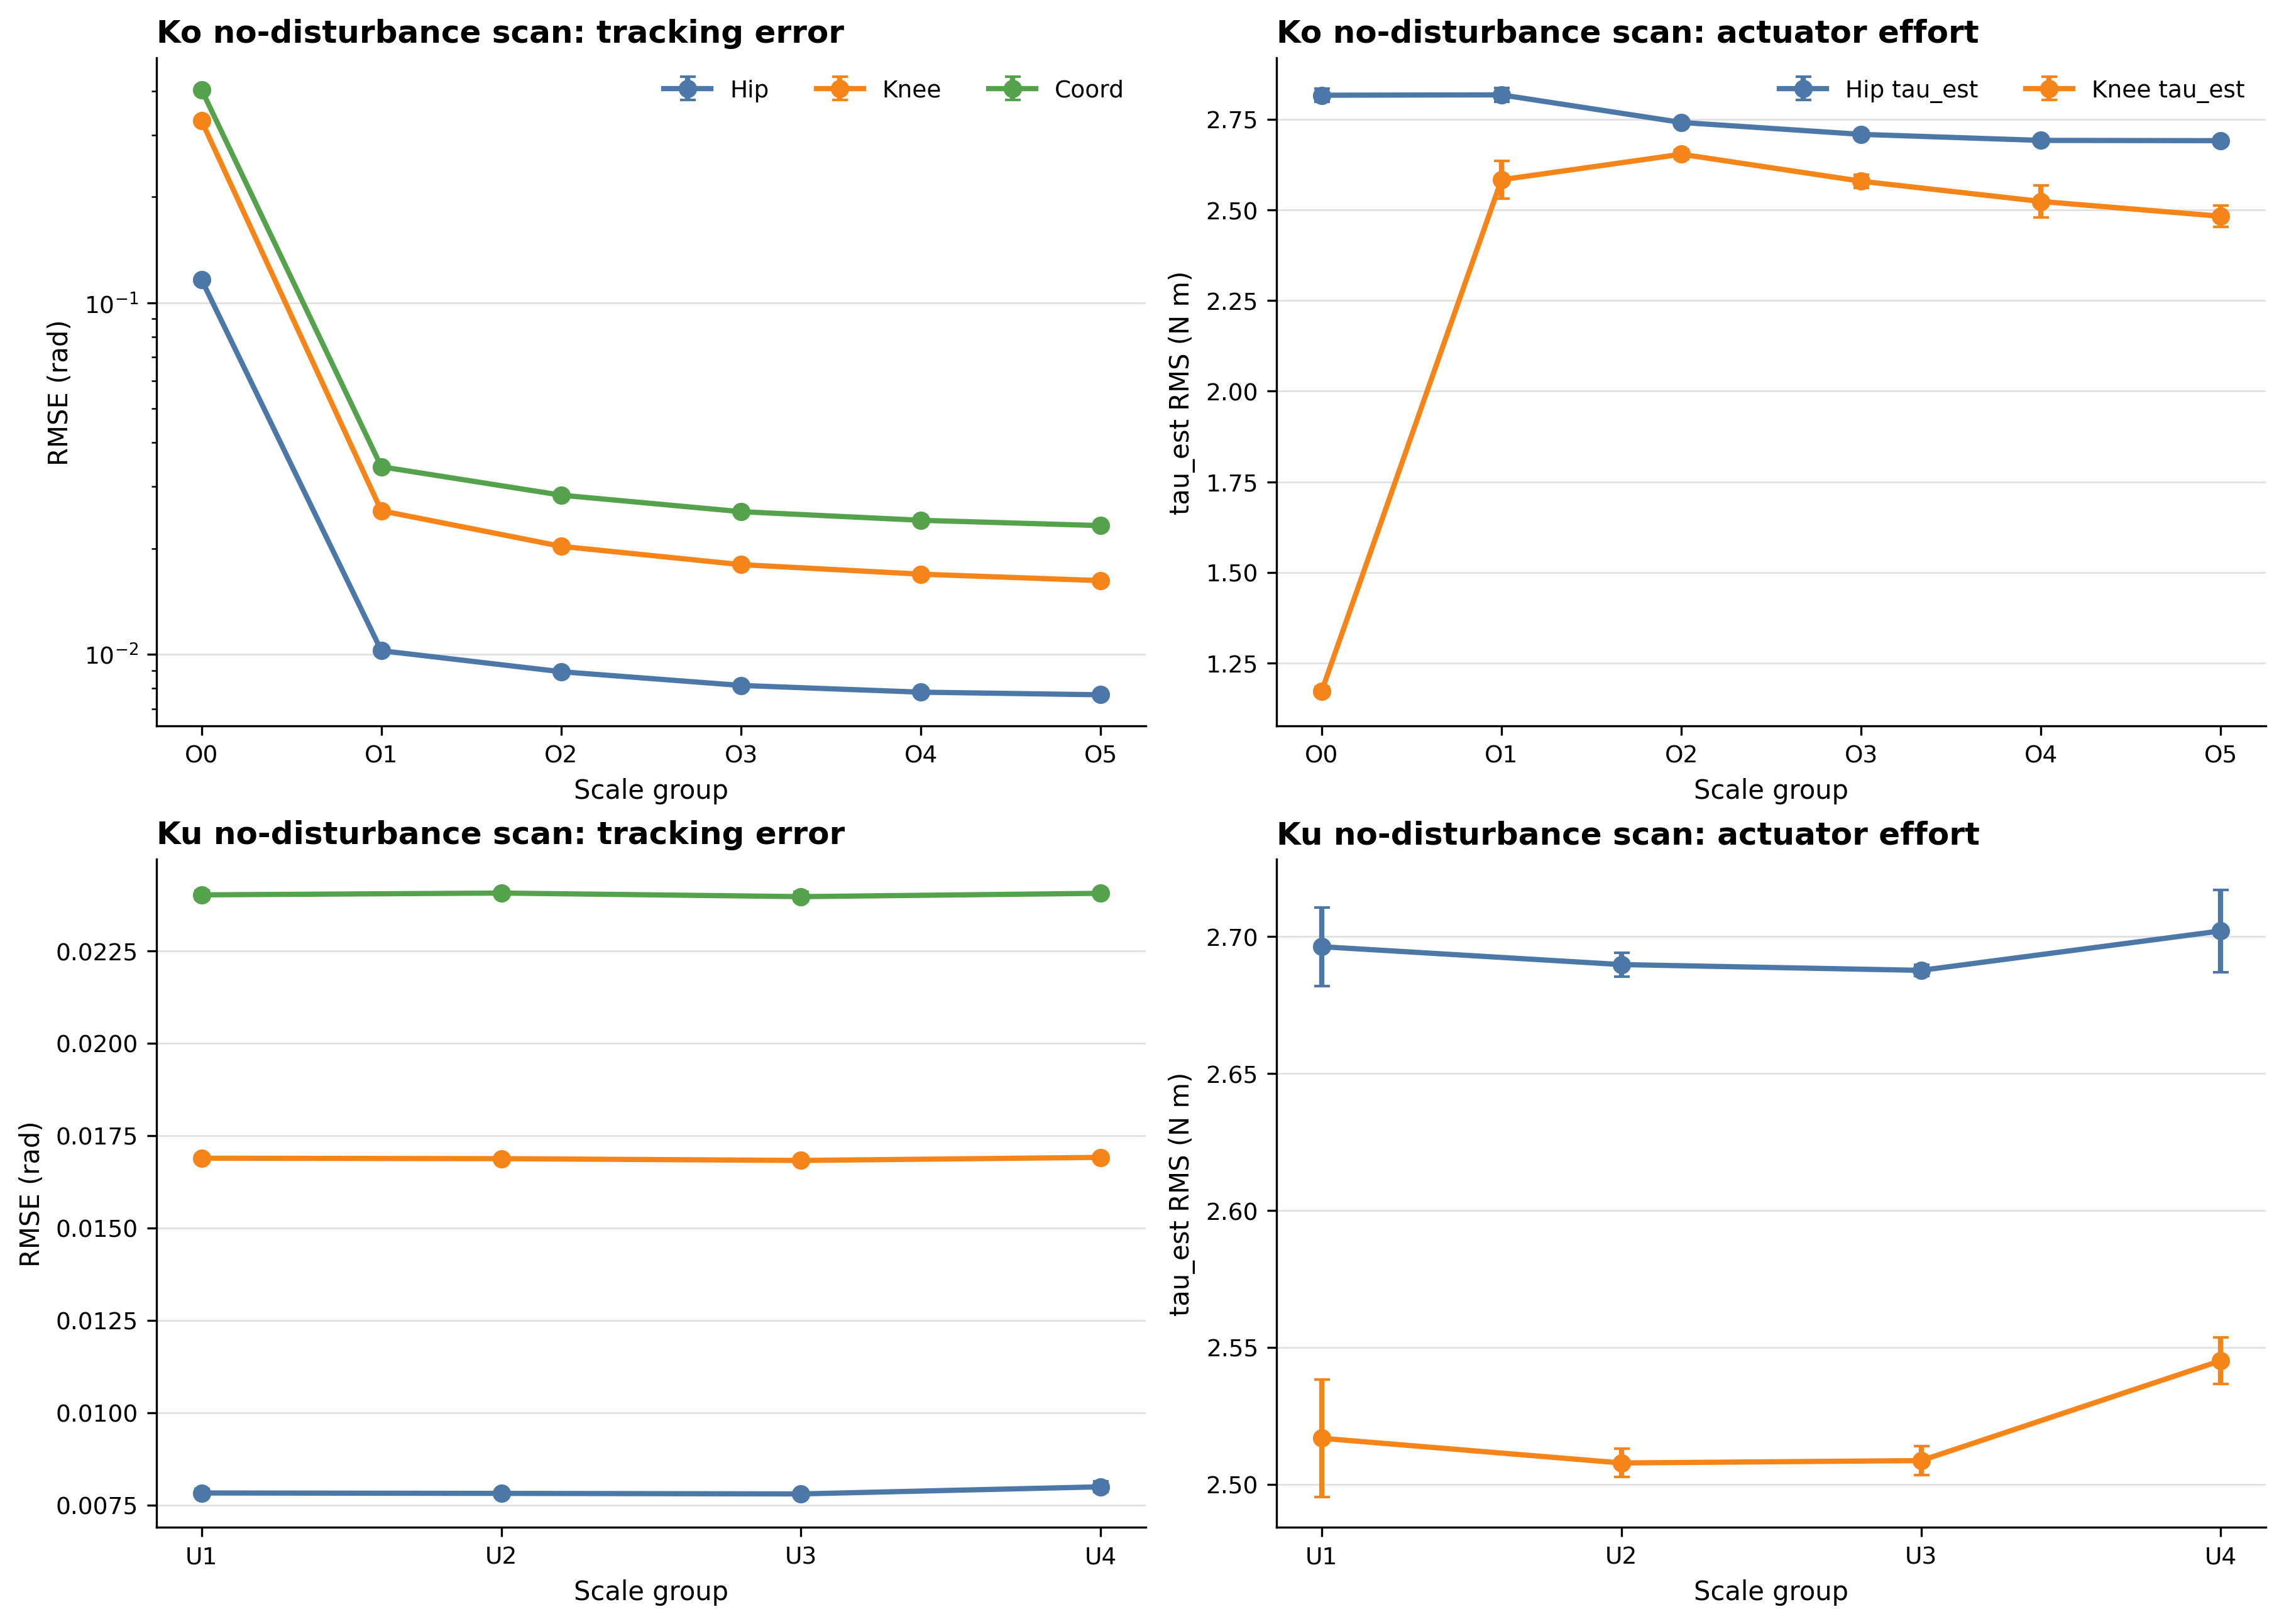
\includegraphics[width=0.92\textwidth]{figures/real_p4_gain_scans.png}
\caption{P4 的 $K_o$ 与 $K_u$ 无扰动扫描。$K_o$ 从 O0 到 O5 降低跟踪误差；$K_u$ 在无扰动条件下对误差影响很小。}
\end{figure}


\subsubsection{$K_o$ 扫描结果}


\begin{table}[htbp]
\centering
\footnotesize
\caption{$K_o$ 无扰动扫描结果}
\begin{tabularx}{\textwidth}{YYYYYYY}
\toprule
组别 & $K_o$ 缩放 & 髋 RMSE rad & 膝 RMSE rad & 协调 RMSE rad & 髋 $\tau_\mathrm{est}$ RMS & 膝 $\tau_\mathrm{est}$ RMS \\
\midrule
O0 & 0.00 & 0.1164 & 0.3295 & 0.4041 & 2.8165 & 1.1723 \\
O1 & 0.25 & 0.0102 & 0.0256 & 0.0341 & 2.8175 & 2.5834 \\
O2 & 0.50 & 0.0089 & 0.0203 & 0.0283 & 2.7415 & 2.6537 \\
O3 & 0.75 & 0.0081 & 0.0180 & 0.0254 & 2.7086 & 2.5793 \\
O4 & 1.00 & 0.0078 & 0.0169 & 0.0240 & 2.6919 & 2.5235 \\
O5 & 1.25 & 0.0077 & 0.0162 & 0.0232 & 2.6911 & 2.4826 \\
\bottomrule
\end{tabularx}
\end{table}


O0 的跟踪误差高于其他组，说明关闭观测器增益后 EID 内部预测与实测之间存在较大偏差。O1 到 O5 的误差随 $K_o$ 增大逐步下降，且 $\tau_\mathrm{est}$ RMS 没有明显恶化。无扰动数据表明，O4/O5 均处于本轮测试覆盖的稳定运行区间；O5 的 RMSE 略低于 O4，但二者差异较小。

\begin{figure}[htbp]
\centering
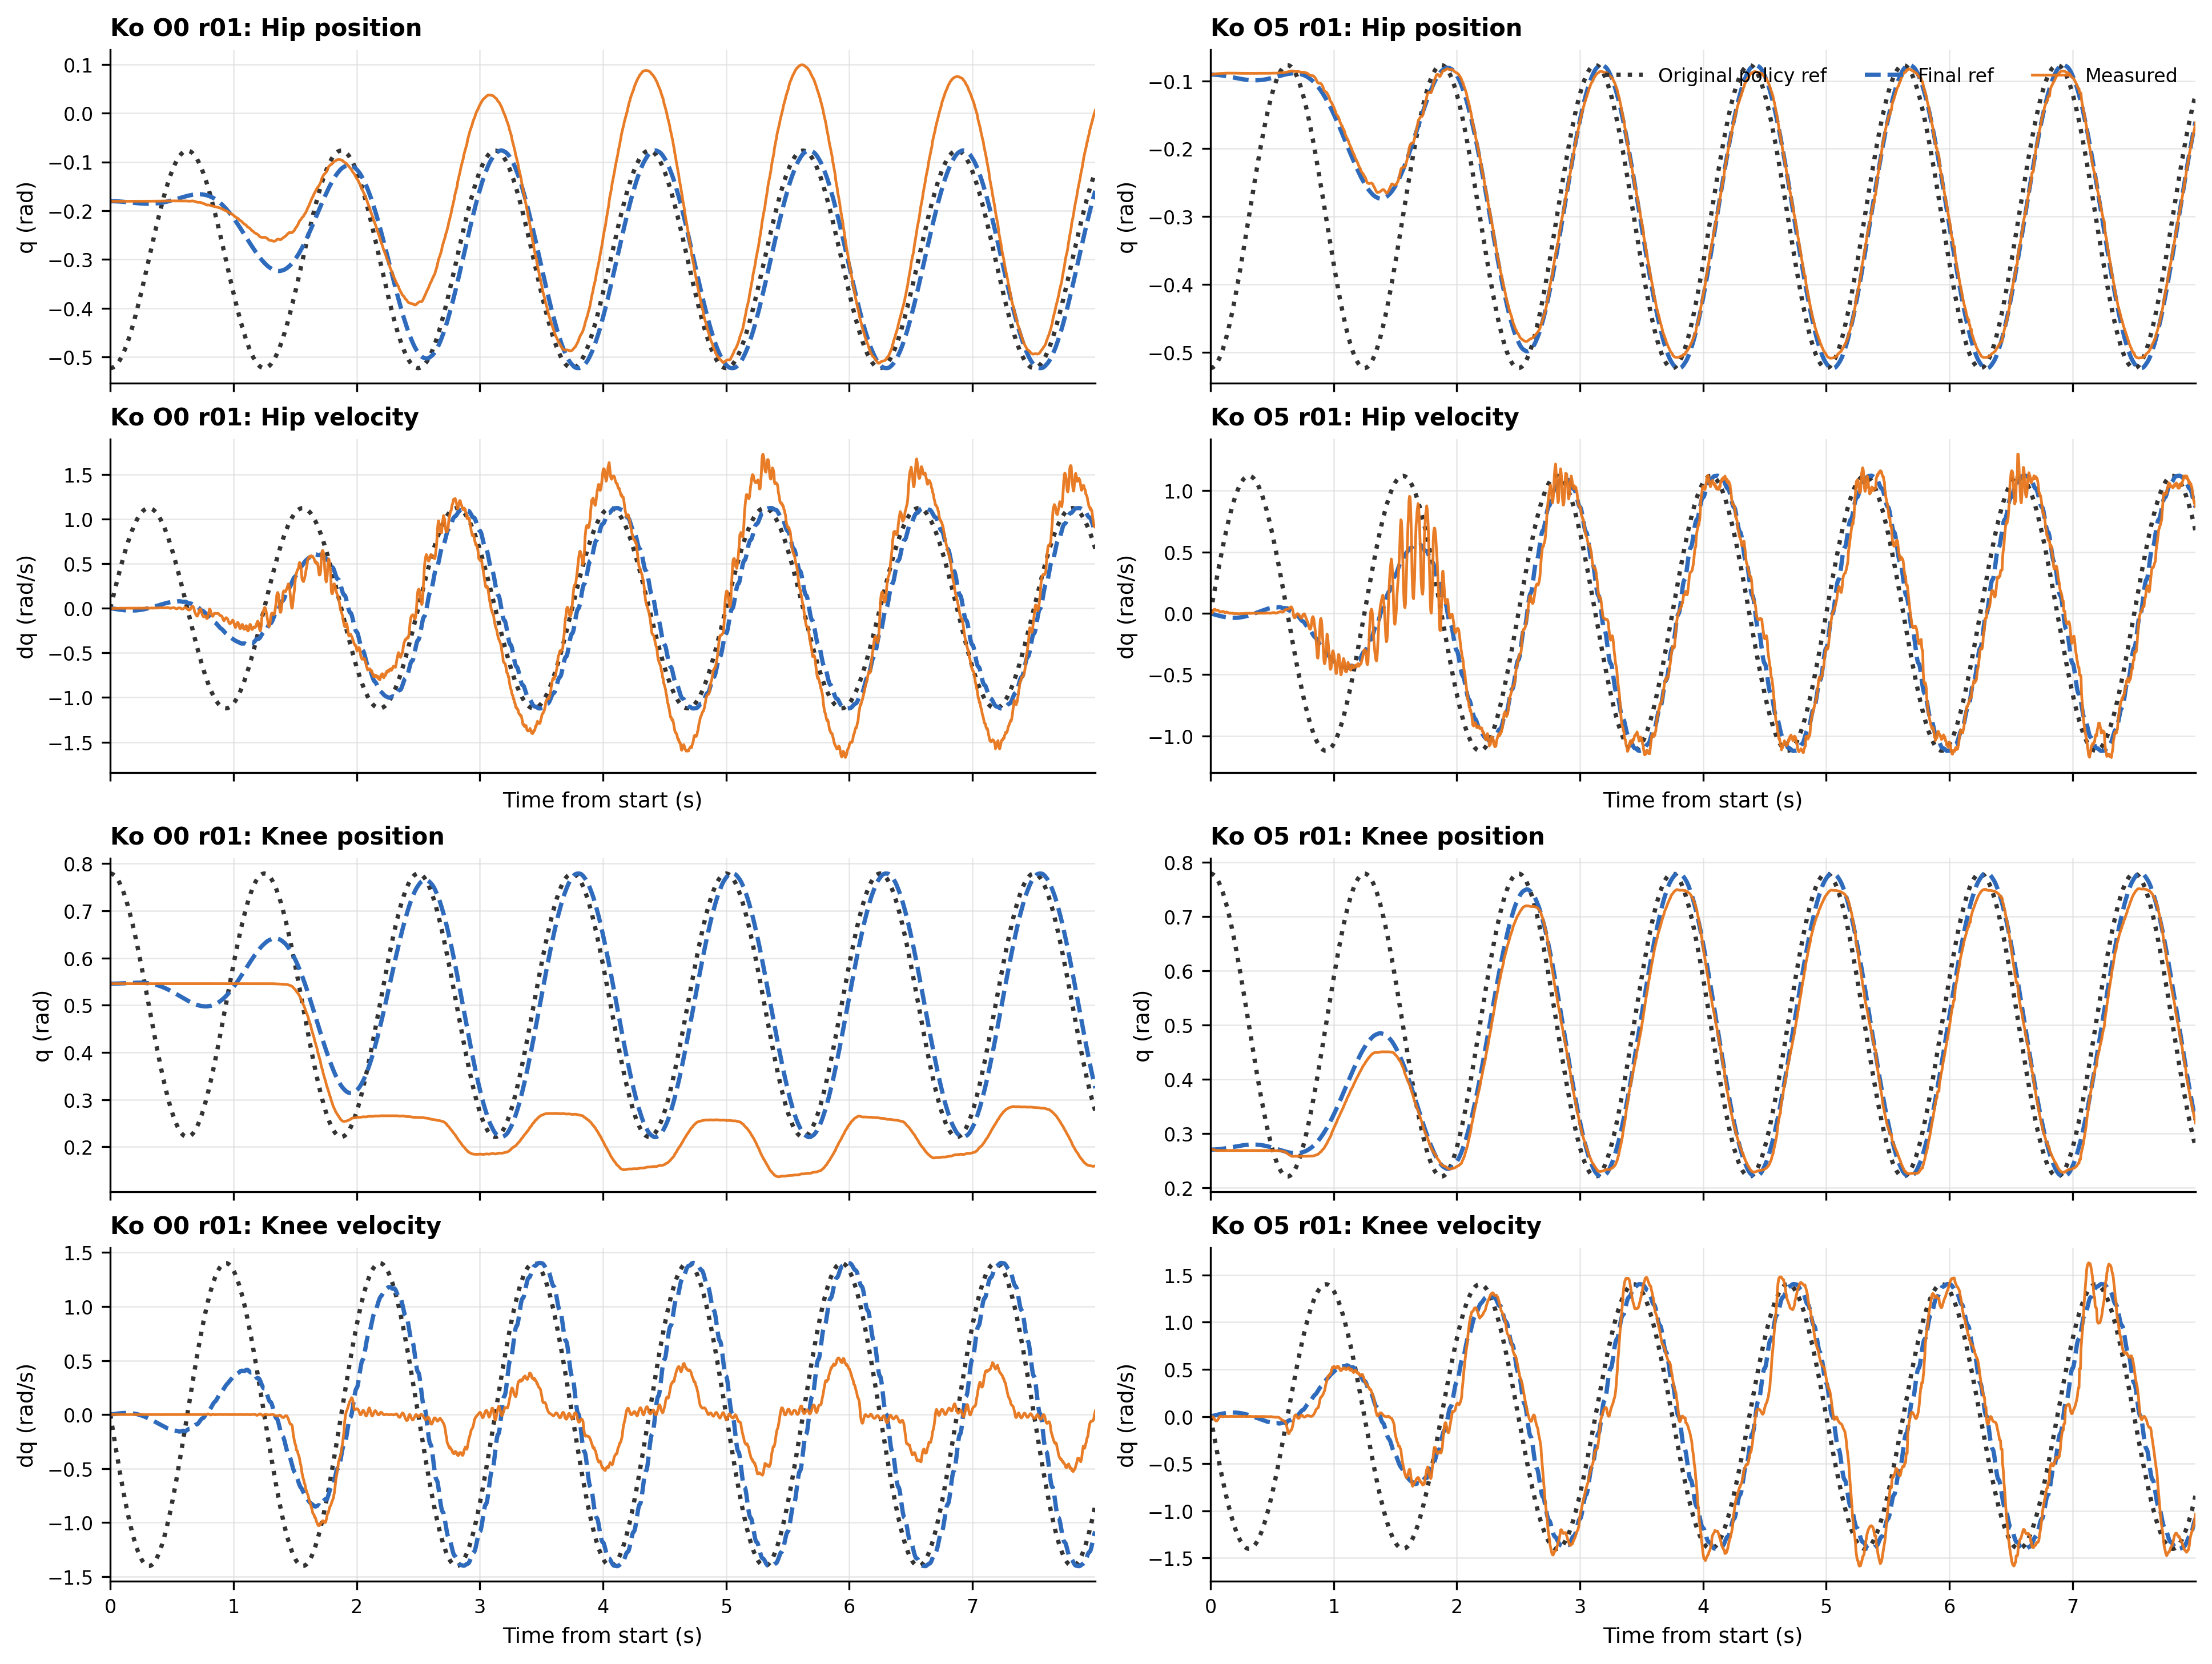
\includegraphics[width=0.92\textwidth]{figures/real_ts_p4_ko_o0_o5_r01.png}
\caption{P4 $K_o$ 最小与最大组的代表性时序，重复 r01。O0 关闭观测器增益后，尤其膝关节位置和速度跟踪明显偏离最终参考；O5 的跟踪误差低于 O0。}
\end{figure}


\subsubsection{$K_u$ 扫描结果}


\begin{table}[htbp]
\centering
\footnotesize
\caption{$K_u$ 无扰动扫描结果}
\begin{tabularx}{\textwidth}{YYYYYYY}
\toprule
组别 & $K_u$ 缩放 & 髋 RMSE rad & 膝 RMSE rad & 协调 RMSE rad & 髋 $\tau_\mathrm{est}$ RMS & 膝 $\tau_\mathrm{est}$ RMS \\
\midrule
U1 & 0.50 & 0.0078 & 0.0169 & 0.0240 & 2.6963 & 2.5168 \\
U2 & 0.75 & 0.0078 & 0.0169 & 0.0241 & 2.6898 & 2.5078 \\
U3 & 1.00 & 0.0078 & 0.0168 & 0.0240 & 2.6877 & 2.5086 \\
U4 & 1.25 & 0.0080 & 0.0169 & 0.0241 & 2.7021 & 2.5451 \\
\bottomrule
\end{tabularx}
\end{table}


$K_u$ 在无扰动条件下几乎不改变跟踪误差，这说明当前 $K_u$ 扫描主要验证了无扰动稳定性，而不是扰动抑制能力。U4 有一次完整日志后的异常返回记录，因此仅凭无扰动结果不能支持提高 $K_u$ 的结论。后文 P4D 使用明确软件扰动窗口进一步比较 U1--U4。

\begin{figure}[htbp]
\centering
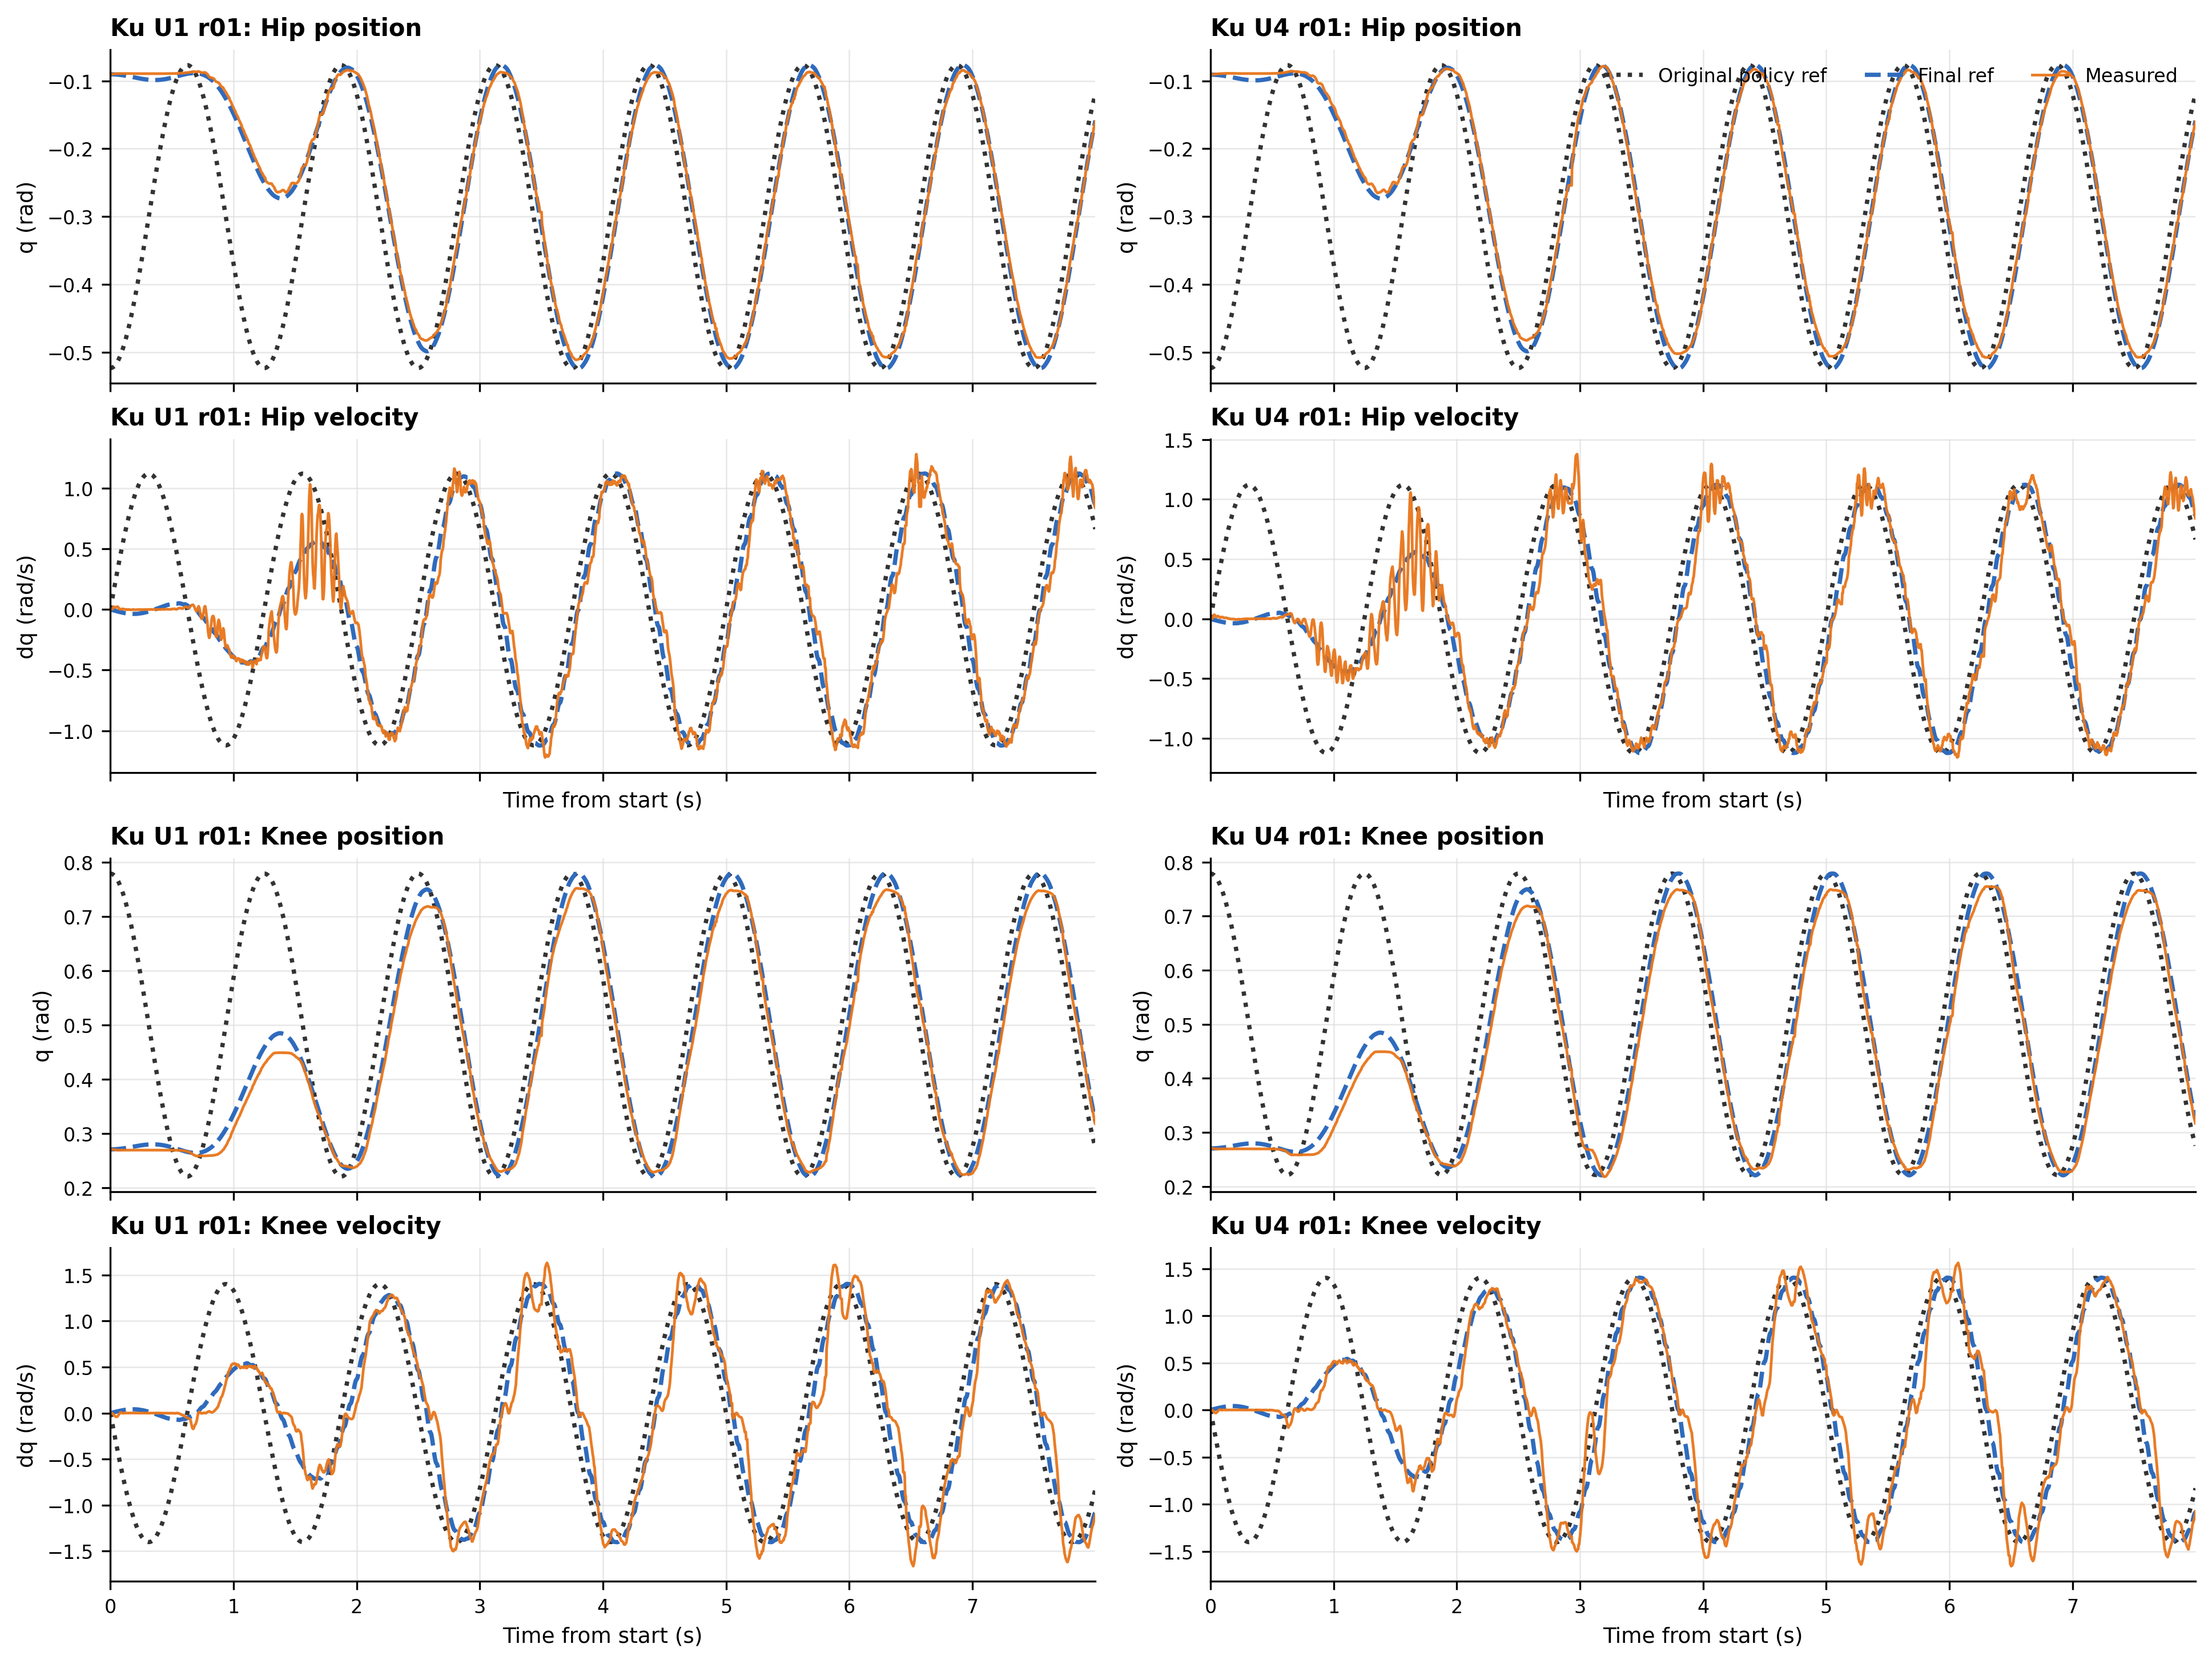
\includegraphics[width=0.92\textwidth]{figures/real_ts_p4_ku_u1_u4_r01.png}
\caption{P4 $K_u$ 最小与最大组的代表性时序，重复 r01。U1 与 U4 在无扰动条件下的时序差异较小，与扫描统计中 $K_u$ 对 RMSE 影响有限的结论一致。}
\end{figure}


\subsection{P4D：带软件扰动的 $K_o$ 与 $K_u$ 扫描}


P4D 使用与 P2D 相同的 $[+6,-4]\ \mathrm{N\cdot m}$ 双关节软件力矩脉冲。该实验直接回答：无扰动下可用的 $K_o/K_u$ 参数，在明确扰动窗口下是否仍稳定，以及增益变化是否真的改善窗口抗扰。

\begin{figure}[htbp]
\centering
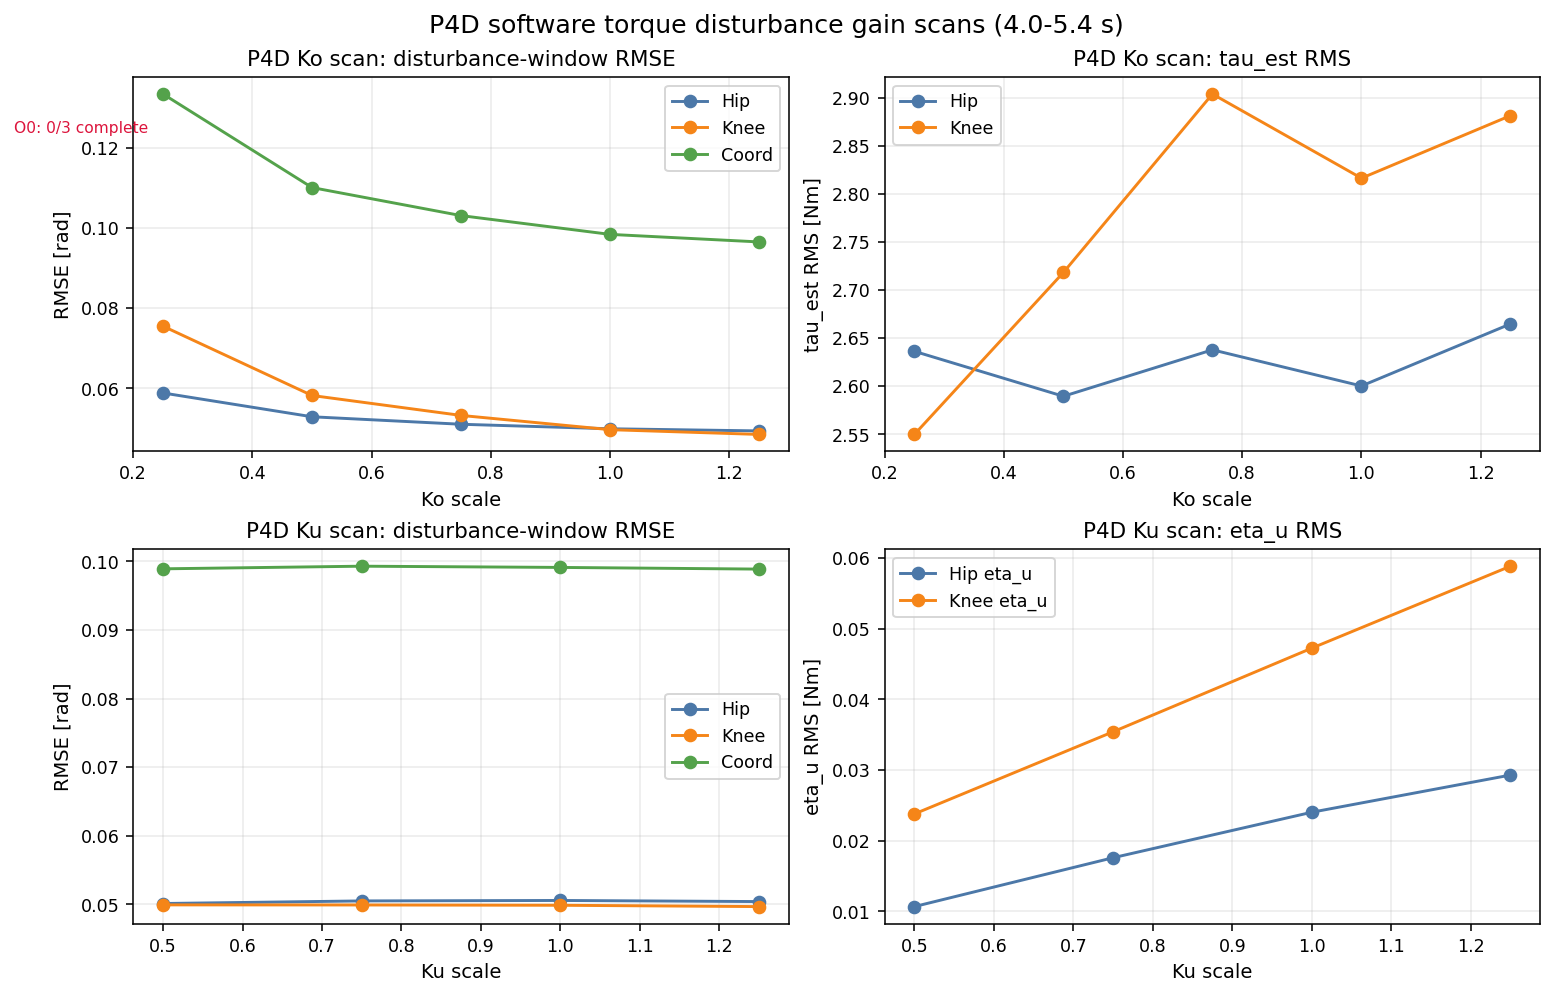
\includegraphics[width=0.92\textwidth]{figures/real_p4d_gain_scans.png}
\caption{P4D 带软件扰动增益扫描。$K_o$ 增大时扰动窗口 RMSE 下降；$K_u$ 扫描中窗口 RMSE 几乎不变，但 $\eta_u$ RMS 随 $K_u$ 增大。}
\end{figure}


\subsubsection{P4D $K_o$ 扫描结果}


\begin{table}[htbp]
\centering
\footnotesize
\caption{P4D $K_o$ 扰动扫描结果}
\begin{tabularx}{\textwidth}{YYYYYYYYY}
\toprule
组别 & $K_o$ 缩放 & 完整运行 & 完整扰动窗口 & 髋窗口 RMSE & 膝窗口 RMSE & 协调窗口 RMSE & 髋 $\tau_\mathrm{est}$ RMS & 膝 $\tau_\mathrm{est}$ RMS \\
\midrule
O0 & 0.00 & 0/3 & 0/3 & - & - & - & - & - \\
O1 & 0.25 & 2/3 & 3/3 & 0.0588 & 0.0755 & 0.1334 & 2.6362 & 2.5498 \\
O2 & 0.50 & 2/3 & 3/3 & 0.0529 & 0.0582 & 0.1101 & 2.5895 & 2.7183 \\
O3 & 0.75 & 2/3 & 3/3 & 0.0510 & 0.0532 & 0.1031 & 2.6378 & 2.9040 \\
O4 & 1.00 & 3/3 & 3/3 & 0.0499 & 0.0497 & 0.0984 & 2.6002 & 2.8164 \\
O5 & 1.25 & 3/3 & 3/3 & 0.0494 & 0.0485 & 0.0965 & 2.6647 & 2.8815 \\
\bottomrule
\end{tabularx}
\end{table}


O0 在三次重复中均于约 4.29 s 结束，未覆盖完整扰动窗口，因此不能计算完整窗口抗扰指标。这一点比无扰动 P4 更严格地说明：关闭观测器增益后，EID 整体结构不具备带扰动可用性。

O1 到 O5 均覆盖完整扰动窗口，且窗口 RMSE 随 $K_o$ 增大逐步下降。O4 和 O5 三次重复均完整跑满 10 s。O5 的窗口误差最低，但相对 O4 的下降幅度较小，同时髋、膝 $\tau_\mathrm{est}$ RMS 略高。该结果说明，在本轮软件扰动条件下，O4 与 O5 构成误差和力矩代价相邻的两组高增益结果，而非单一最优结论。

\subsubsection{P4D $K_u$ 扫描结果}


\begin{table}[htbp]
\centering
\footnotesize
\caption{P4D $K_u$ 扰动扫描结果}
\begin{tabularx}{\textwidth}{YYYYYYYY}
\toprule
组别 & $K_u$ 缩放 & 完整运行 & 髋窗口 RMSE & 膝窗口 RMSE & 协调窗口 RMSE & 髋 $\eta_u$ RMS & 膝 $\eta_u$ RMS \\
\midrule
U1 & 0.50 & 3/3 & 0.0501 & 0.0499 & 0.0989 & 0.0107 & 0.0238 \\
U2 & 0.75 & 3/3 & 0.0505 & 0.0499 & 0.0993 & 0.0176 & 0.0354 \\
U3 & 1.00 & 3/3 & 0.0506 & 0.0499 & 0.0991 & 0.0240 & 0.0473 \\
U4 & 1.25 & 3/3 & 0.0504 & 0.0497 & 0.0989 & 0.0293 & 0.0589 \\
\bottomrule
\end{tabularx}
\end{table}


$K_u$ 扫描与无扰动 P4 的结论一致：在当前扰动幅值下，改变 $K_u$ 几乎不改变髋、膝或协调窗口 RMSE。不同的是，P4D 明确显示 $\eta_u$ RMS 随 $K_u$ 增大而上升。也就是说，在本轮软件扰动条件下，提高 $K_u$ 主要增加补偿量活动，而没有带来可辨识的窗口 RMSE 收益。

\textbf{P4D 参数建议。} 本轮不支持继续增大 $K_u$。U1--U4 的窗口 RMSE 几乎重合，而 $\eta_u$ RMS 随 $K_u$ 增大，因此提高 $K_u$ 主要增加补偿量活动，并未带来可辨识的窗口误差收益。下一轮建议固定两组候选参数：\textbf{O4+U1 作为主推荐参数，O5+U1 作为备选参数}。O4 的力矩代价较低，O5 的窗口误差略低但力矩 RMS 略高。

\section{讨论}


\subsection{EID 整体结构的有效性与代价}


P1、P2-H 和 P2D 共同表明，EID 整体结构在本轮右髋-右膝台架实验中降低了多项误差指标。P1 支持无扰动门槛验证，P2-H 支持人工扰动工况下的全稳态统计改善，P2D 支持软件输入端等效扰动窗口下的部分抗扰收益。与此同时，EID 整体结构的力矩变化量增加也很明确，因此后续必须以“误差收益--力矩代价”共同评价算法，而不能只报告 RMSE。

\subsection{证据边界}


本轮证据分为三类。第一类是无扰动稳态跟踪结论，主要来自 P1/P4。第二类是人工扰动全稳态统计结论，来自 P2-H，但由于没有扰动时间戳，不能计算扰动窗口指标。第三类是软件输入端等效扰动结论，来自 P2D/P4D，其扰动时间和幅值可复现，但该扰动不等价于外部物理接触力。因此，本轮尚未完成真实物理外扰抗扰验证。

\subsection{参数与下一步方向}


参数结果显示，O0 不满足带扰动可用性；O4/O5 是本轮稳定性和误差表现较好的候选区间。$K_u$ 扫描没有显示额外 RMSE 收益，因此下一步不应继续大范围提高 $K_u$。在进入新的上机实验前，应先用现有 P2D/P4D 日志比较 O4+U1 与 O5+U1 的频谱代价，并通过消融仿真、增广闭环频响和残差定义比较解释当前结构的主要性能杠杆。

\section{结论}


本轮实验得到以下结论：

\begin{enumerate}[label=\arabic*.]
\item \textbf{EID 整体结构通过无扰动门槛验证。} 在 P1 低幅双关节台架实验中，EID 相对 PD 降低髋、膝和协调 RMSE，且未观察到批量运行失败。
\item \textbf{EID 整体结构在软件输入端等效扰动下表现出部分抗扰收益。} 在 P2D $[+6,-4]\ \mathrm{N\cdot m}$ 软件力矩扰动窗口中，EID 降低髋窗口 RMSE 18.2\%、协调窗口 RMSE 6.1\%，但膝窗口 RMSE 上升 10.0\%。因此，本轮不能写成“所有扰动指标均改善”。
\item \textbf{EID 整体结构的主要代价是力矩活动增加。} P1/P2-H/P2D 均显示 EID 整体结构的 $\Delta\tau_\mathrm{est}$ RMS 上升；P4D 进一步显示，提高 $K_u$ 会放大 $\eta_u$ RMS，但几乎不改善窗口 RMSE。
\item \textbf{Preview-MPC 2 点参考可降低参考激励和力矩变化量。} P3 中 preview2 显著降低参考加速度、参考 jerk 和 $\Delta\tau_\mathrm{est}$ RMS，同时只带来小幅跟踪 RMSE 上升。
\item \textbf{参数上建议保留 O4+U1 和 O5+U1。} O0 不满足带扰动可用性；O4/O5 均能完成 P4D 完整重复。由于增大 $K_u$ 没有带来明确 RMSE 收益，下一轮不建议继续大范围提高 $K_u$。
\item \textbf{本轮结论不等同于真实物理外扰结论。} P2D/P4D 属于输入端等效扰动实验，不能替代外部物理接触力实验。真实物理外扰抗扰能力需在下一轮用可测外力方式验证。
\end{enumerate}


\section{后续工作}


后续工作分为两类。第一类是基于现有 P2D/P4D 实物日志的离线分析，不需要再次上机器人，风险低，直接补齐本文关于力矩变化量增加和恢复段行为的证据链。第二类是面向控制器本体的仿真与机理分析，用于解释 EID 整体结构究竟通过哪条通道降低误差、为什么 $K_u$ 扫描收益有限，以及如何把 O4/O5 这类经验参数转化为有带宽和稳定裕度解释的设计。

\subsection{P2D/P4D 频谱分析}

当前结果已经说明 EID 的主要代价是 $\Delta\tau_\mathrm{est}$ RMS 增加，而不是平均力矩 RMS 大幅上升。下一步应进一步回答力矩变化集中在哪些频段，并区分正常跟踪频谱与扰动响应频谱。

\begin{table}[htbp]
\centering
\footnotesize
\caption{P2D/P4D 频谱分析信号与目的}
\begin{tabularx}{\textwidth}{YY}
\toprule
信号 & 目的 \\
\midrule
$\tau_\mathrm{est}$ 频谱 & 判断执行器力矩是否出现高频成分 \\
$\Delta\tau_\mathrm{est}$ 频谱 & 判断力矩粗糙度主要来自哪个频段 \\
$\eta_u$ 频谱 & 判断 EID 补偿是否在高频放大 \\
$q/\dot q$ 误差频谱 & 判断误差改善是否伴随高频抖动 \\
扰动窗口 vs 非扰动窗口 & 区分正常跟踪引起的频谱和扰动响应引起的频谱 \\
\bottomrule
\end{tabularx}
\end{table}

建议输出两张图。第一张为 PD vs EID 的 $\tau_\mathrm{est}$ 与 $\Delta\tau_\mathrm{est}$ 频谱对比，用于说明 EID 的力矩代价是否集中在高频。第二张为 O4+U1 vs O5+U1 的 $\eta_u$ 与 $\tau_\mathrm{est}$ 频谱对比，用于判断 O5 的小幅误差收益是否伴随更强的高频力矩。如果 O5 的误差只比 O4 略低，但高频力矩明显更强，则下一轮应坚定选择 O4+U1 作为主参数。

\subsection{恢复段统计补充}

P2D/P4D 的扰动窗口统计已经较清楚，但恢复段尚未完全闭环。本文定义恢复观察段为 $5.4$--$7.4\ \mathrm{s}$，统计时只纳入完整覆盖该时间段的日志；未覆盖完整恢复窗口的日志只用于扰动窗口结论，不用于恢复段均值。

\begin{table}[htbp]
\centering
\footnotesize
\caption{恢复段补充统计指标}
\begin{tabularx}{\textwidth}{YY}
\toprule
指标 & 含义 \\
\midrule
恢复 RMSE & 扰动结束后是否快速回到参考 \\
恢复峰值误差 & 扰动撤除瞬间是否有反冲 \\
恢复时间 & 误差回到阈值内需要多久 \\
恢复段 $\Delta\tau_\mathrm{est}$ RMS & 回稳是否依赖高频力矩快速拉回 \\
\bottomrule
\end{tabularx}
\end{table}

该分析用于判断控制器是否只在扰动窗口内表现较好，却在扰动撤除后产生较大反冲或较慢回稳。对于后续真实物理外扰实验，这一项直接关系到安全性。

\subsection{控制器机理拆解与消融仿真}

仿真计划首先不应把 EID 整体结构当作黑箱。当前控制律中，$\eta_k$ 同时进入中心反馈状态修正路径和输入补偿路径：

\[
u_k=u_k^*-\eta_{u,k}+K(r_k-\bar{x}_k),
\qquad
\bar{x}_k=\hat{x}_k+\eta_k
\]

因此，误差下降可能来自解析逆模型前馈、中心反馈状态修正、输入端补偿，或三者耦合。下一步应在仿真中构造四个消融版本，分别隔离各通道贡献。

\begin{table}[htbp]
\centering
\footnotesize
\caption{EID 整体结构消融仿真版本}
\begin{tabularx}{\textwidth}{YY}
\toprule
版本 & 控制律目的 \\
\midrule
A：解析逆模型 + 普通 PD & 只看 $u^*$ 的贡献 \\
B：解析逆模型 + 中心反馈状态，且 $\eta_u=0$ & 只看 $\bar{x}=\hat{x}+\eta$ 的贡献 \\
C：解析逆模型 + 输入补偿，反馈仍用实测状态 & 只看 $-\eta_u$ 的贡献 \\
D：当前完整 EID & 与前三者比较整体收益和力矩代价 \\
\bottomrule
\end{tabularx}
\end{table}

该消融用于回答当前结构的核心问题：P4D 中提高 $K_u$ 几乎不改善窗口 RMSE，却明显放大 $\eta_u$ RMS，这是否说明当前收益主要来自 $K_o$ 触发的状态修正和反馈重构，而不是有效的输入端力矩补偿。

\subsection{离散时间增广闭环与频响分析}

第二步应把控制器写成离散时间增广闭环系统，而不是只报告哪个参数的 RMSE 更小。可从单关节线性化模型开始，将真实状态、标称预测状态和 EID 估计量并入增广状态：

\[
X_k=
\begin{bmatrix}
x_k\\
\hat{x}_k\\
\eta_k
\end{bmatrix},
\qquad
X_{k+1}=A_{cl}X_k+B_r r_k+B_d d_k+B_v v_k+B_w w_k
\]

在该框架下，O4/O5 的差异应被解释为闭环极点、扰动抑制带宽、噪声到力矩增益和参考到力矩增益的差异，而不是单纯的经验参数优劣。

\begin{table}[htbp]
\centering
\footnotesize
\caption{增广闭环仿真分析图}
\begin{tabularx}{\textwidth}{YY}
\toprule
图或分析 & 目的 \\
\midrule
$K_o,K_u,\alpha$ 网格下的闭环极点图 & 判断稳定裕度 \\
扰动 $d\rightarrow e$ 的频响 & 判断抗扰带宽 \\
测量噪声 $v\rightarrow u$ 的频响 & 判断噪声放大 \\
参考 $r\rightarrow u$ 的频响 & 判断参考激励如何进入力矩 \\
扰动 $d\rightarrow \eta_u$ 的频响 & 判断 EID 补偿是否真的跟随扰动 \\
\bottomrule
\end{tabularx}
\end{table}

这一步的目标是把“经验上 O4/O5 能跑”转化为“参数具有明确带宽、稳定裕度和噪声放大解释”。

\subsection{残差定义与 $K_u$ 通道可辨识性}

当前实现中，EID 更新使用的是 $x_k-\bar{x}_k$，而不是 $x_k-\hat{x}_k$。由于 $\bar{x}_k=\hat{x}_k+\eta_k$，当前残差等价于

\[
x_k-\bar{x}_k=x_k-\hat{x}_k-\eta_k
\]

这会形成估计量自反馈，使 $\eta_k$ 更像带泄漏的误差滤波器，而不一定是纯扰动估计器。仿真中应比较两种残差定义，并可进一步引入混合残差：

\[
e_{\eta,\lambda}=x_k-\hat{x}_k-\lambda\eta_k
\]

其中 $\lambda=1$ 是当前版本，$\lambda=0$ 是标称预测残差版本。

\begin{table}[htbp]
\centering
\footnotesize
\caption{残差定义与输入补偿通道分析}
\begin{tabularx}{\textwidth}{YY}
\toprule
分析项 & 目的 \\
\midrule
闭环极点比较 & 判断哪种残差定义稳定裕度更大 \\
$\eta_u$ 与已知软件扰动 $\tau_d$ 的相关性、幅值比和相位差 & 判断 $\eta_u$ 是否像真实输入扰动估计 \\
噪声到力矩增益 & 判断哪种残差定义更容易放大高频 \\
扰动结束后的恢复 & 判断哪种残差定义反冲更小 \\
$u_k^*$、$-\eta_{u,k}$、$K(r_k-\bar{x}_k)$ 的 RMS 和频谱占比 & 判断当前 EID 的实际作用主要来自输入补偿还是反馈中心改变 \\
\bottomrule
\end{tabularx}
\end{table}

如果 $\eta_u$ 与已知软件扰动低相关、相位滞后大，且提高 $K_u$ 只是放大内部活动而不降低 RMSE，则说明 $K_u$ 在当前结构中不是主要性能杠杆。此时应优先研究残差定义和反馈中心构造，而不是继续扩大 $K_u$ 扫描范围。

\subsection{误差收益--力矩代价的多目标仿真设计}

最后，应把本文反复出现的“误差收益--力矩代价”写成正式多目标设计问题，而不是单一 RMSE 优化。一个可用的仿真目标函数为：

\[
\begin{aligned}
J=&
w_1 \mathrm{RMSE}_{hip}
+w_2 \mathrm{RMSE}_{knee}
+w_3 \mathrm{RMSE}_{coord}\\
&+w_4 \mathrm{RMS}(\tau)
+w_5 \mathrm{RMS}(\Delta \tau)
+w_6 \mathrm{RMS}(\eta_u)
+w_7 N_{\mathrm{sat}}
\end{aligned}
\]

建议输出 Pareto 前沿图：横轴为扰动窗口协调 RMSE，纵轴为 $\Delta\tau_\mathrm{est}$ RMS，点颜色表示 $K_o$，点大小表示 $K_u$ 或 $\eta_u$ RMS。该图应明确 O4+U1 是否是保守 Pareto 点、O5+U1 是否是更激进的 Pareto 点，以及高 $K_u$ 是否属于力矩代价更大但误差不更低的 dominated solution。


\end{document}
